
\documentclass{beamer}
\usepackage[spanish]{babel}
\usepackage[utf8]{inputenc}
\usepackage[style=american]{csquotes}
\usepackage{lmodern}
\uselanguage{spanish}
\languagepath{spanish}


\def\tituloTesis{Hacia un método computacional para detectar léxico contrastivo}

\title{\tituloTesis}
\author{Damián Eliel Aleman}

\usetheme{Madrid}
\usecolortheme{beaver}


\begin{document}

\beamertemplatenavigationsymbolsempty


\AtBeginSection[]
{

\begin{frame}
\frametitle{Temario}
\tableofcontents[
currentsection,
]
\end{frame}

}

\frame{\titlepage}

\section{Introducción}
%Explicación del área
%el trabajo de vidal de batini y almeida
%Objetivo de la tesis

%Contrsuccion de lingüistica de corpus
%lingüistica computacional, su evolucion
%Todo se hace en ingles y hay pocos analisis en castellano.

%primer acercamiento de contrastes léxicos 


%Comentar el problema de la lingüística de Corpus, trabajo previo en el área, comentar brevemente qué queremos hacer. Acá va a ir mucho de lo que nos pasó Santiago como literatura, incluso mencionando (por ejemplo) el trabajo de Vidal de Battini

\section{Trabajo previo en el área}
La dialectología es un campo que estudia la variación de las lenguas según la región geográfica. La investigación en estos campo suele utilizar variables lingüísticas: atributos fonéticos, sintácticos y léxicos.

%Ampliar sobre dialectologia (fijarse en la enciclopedia)
Una palabra es \textit{contrastiva} cuando la frecuencia de uso en dos regiones es muy diferente. Por ejemplo, la palabra ``che''\footnote{Tratamiento que se usa para llamar, pedir atención o dirigirle a alguien la palabra \cite{academia2008diccionario}.}, o ``metegol''\footnote{Juego mecánico en el que con pequeños muñecos se simula un partido de fútbol (futbolín) \cite{academia2008diccionario}.} son términos más usados en la Argentina que en España. Un ejemplo dentro de la Argentina, es el de ``gurisada'' conocido en el litoral y noroeste argentino como un conjunto de chicos \cite{academia2008diccionario}.
%El criterio de contrastividad es importante especialmente para realizar diccionarios contrastivos como el 
Actualmente, las palabras con contraste léxico en distintas regiones
se detectan por medio de cuestionarios como el de \emph{Almeida} \cite{almeida1995variacion} o en métodos que dependen, en mayor o menor medida, de la intuición y sensibilidad de los lexicógrafos. Las encuestas están integradas por grupos temáticos centrales como la casa, la familia, la enseñanza, el cuerpo humano, etc. Sobre cada grupo temático se les indica a las personas entrevistadas un repertorio de palabras por cada noción, para ver si las conocen y con qué frecuencia se las usa. 
Con el presente trabajo planteamos cambiar el paradigma y detectar automáticamente las palabras usadas en distintas regiones y sus frecuencias.

Uno de los corpus lingüísticos del español más reconocidos es el \emph{CORPES XXI}\cite{espanolabanco}, creado por la Real Academia Española con una distribución de 25 millones de formas por cada uno de los años comprendidos en el periodo 2001 
a 2012. Sin embargo, dicho corpus tiene dos desventajas importantes: por un
lado, la cantidad de palabras de América Latina está subrepresentada en relación a la demografía ya que el $34,30$\% de las palabras del dataset proviene de textos de España y $65,70$\% de los demás países hispanoparlantes. Por otro lado, uno no dispone de todo el dataset, sino que solamente se pueden hacer las consultas desde su página web. Estas consultas están limitadas en cuanto a la cantidad de solicitudes y a las funcionalidades que estas proveen, especialmente tener que saber de antemano la forma a buscar.

Una de las virtudes de hacer un corpus con un método de recolección de textos de forma automática se desprende del mayor tamaño del corpus en comparación con métodos manuales como digitalización de textos. A pesar de haber comenzado hace varias décadas la recolección de textos de la web para realizar corpus, no hay muchos en el idioma español.
Uno es el de \textit{Mark Davies}, en el cual se utilizaron las páginas web para recolectar los textos, con dos mil millones de palabras en español, y se dividieron las páginas a partir del país de origen identificado por \textit{Google} \cite{davies2015}. A pesar de ser un corpus muy grande con anotaciones, no permite diferenciar las frecuencias de las palabras o los textos originados en regiones dentro de cada país. Es por eso que para este trabajo elegimos construir nuestro propio conjunto de datos que contenga una gran cantidad de palabras. Para esta tarea, usamos datos de \textit{Twitter}. A continuación haremos una descripción de esta plataforma y de sus principales ventajas sobre otras alternativas posibles.


\section{Twitter}
Twitter\footnote{www.twitter.com} es un servicio de microblogging creado en 2006. Los usuarios son variados, desde personas, instituciones gubernamentales y no gubernamentales hasta bots (i.e programas que corren tareas automáticamente). Cada usuario puede escribir textos llamados tuits, que tienen una longitud máxima de 140 caracteres\footnote{Recientemente han aumentado el límite a los 280 caracteres.}. Las relaciones en Twitter no necesitan ser recíprocas. Es decir, uno puede seguir a una persona en cuyo caso va a poder leer todos los tuits generados por ella, como también puede ser seguido por una persona. Un tuit puede ser respondido, como también puede ser retuiteado. El retuit es un mecanismo para diseminar por la red tuits generados por otros usuarios. De esta manera si un usuario $A$ realiza un retuit generado por el usuario $B$, cualquier seguidor de $A$ también va a recibir ese tuit en su panel, al cual llamaremos \textit{timeline}. Si bien los tuits que se ven en el timeline son solo aquellos generados por los usuarios que uno sigue, todos los tuits son públicos, es decir que se pueden acceder a ellos a través de búsquedas en la plataforma.
Para dar una noción de la cantidad de usuarios en la Argentina, en el año 2016 había 11,8 millones de usuarios de Twitter. Teniendo en cuenta que en ese momento 15 millones de personas tenían smartphones se deduce que el $70$\% de la gente con smartphones poseía una cuenta de Twitter.%{ref de lanacion}

Las ventajas de Twitter sobre otras plataformas son varias: provee una interfaz pública para obtener tuits de cualquier persona, independientemente de que haya una relación con el usuario que escribió los tuits en la red social. Es decir, uno puede ver los tuits de otra persona, sin necesidad de ser un \textit{seguidor} de la misma. Además, a diferencia de un portal de noticias donde los comentarios suelen estar relacionados con estas, en Twitter son más amplios los tópicos de los comentarios.
Por otro lado, Twitter es una tecnología que permite hacer escalable el trabajo a diferentes países ya que con una misma interfaz se pueden obtener los textos de cualquier región. En cambio, si se elige un portal de noticias para sacar comentarios de usuarios, es necesario conocer la estructura de cada página para obtener esos datos.
Otra virtud de Twitter es la identificación de los usuarios sobre la cual se podrían inferir datos como género, edad y ubicación de cada uno.
Por último, una ventaja sobre otro método de recolección es que a través de Twitter se pueden recolectar palabras con una granularidad regional muy variable y obtener información de quienes los escriben.
Existen otras redes sociales de las que se podrían obtener textos para analizar, pero tienen la desventaja de ser privadas, como \textit{Facebook}, o acotadas en términos de los temas que se hablan, como \textit{Linkedin}. 

En los últimos años se han publicado numerosos trabajos que utilizaron datos de Twitter, desde la detección y monitoreo de terremotos en tiempo real\cite{sakaki2010earthquake}, análisis de sentimientos y de la opinión pública \cite{liu2012sentiment},  predicciones del mercado de valores \cite{pak2010twitter} o los resultados de elecciones nacionales \cite{tumasjan2010predicting}. También se ha utilizado para localizar enfermedades por región \cite{paul2011you}.

En cuanto a trabajos relacionados con la lingüística cabe mencionar el trabajo de Eisenstein et al. \cite{eisenstein2010latent} en el que identifica palabras con una gran afinidad regional realizando un modelo probabilístico en el que asumen que las distribuciones léxicas dependen de la región geográfica y de una división de tópicos. En otras palabras, suponen que hay una división de temas sobre todo el dataset y dependiendo de la región del autor, este es más propenso a escribir con una variación dada. El mismo autor realizó un trabajo para identificar variables léxicas y detectar regiones dialectales \cite{eisenstein2014identifying}.
El trabajo de Gonçalves et al. \cite{gonccalves2014crowdsourcing} consistió en analizar las variaciones diatópicas de ciertos conceptos en las grandes ciudades hispanoparlantes. Utilizaron la técnica K-means \cite{bishop2006pattern} para obtener regiones dialectales. Por otro lado G. Doyle et al. \cite{doyle2014mapping} propone un método bayesiano para estimar la distribución de la frecuencia de una palabra (o frase) condicional a la ubicación de la persona que la escribe.
Hay dos grandes diferencias entre el presente trabajo con los que se mencionaron anteriormente. La primera diferencia es que el análisis está hecho sin un enfoque bayesiano. La segunda diferencia es que este trabajo se realizó con textos en español, mientras que la mayoría de los trabajos están hechos sobre corpus en inglés. 


\section{Lingüística de Corpus y Lingüística computacional} % (fold)
\label{linguistica_computacional}

La lingüística de corpus es una rama de la lingüística que investiga a través de conjuntos de muestras de uso de la lengua \cite{mcenery2011corpus}. Aunque lo más común es que estas muestras provengan de textos, también se puede extraer datos a partir de grabaciones de voz o videos. Si bien esta rama nació analizando corpus de forma manual, el rápido crecimiento
tecnológico de las últimas décadas dio la posibilidad de tener corpus con millones de palabras y hacer algunos estudios de manera más automatizada, usando menos recursos humanos y ahorrando tiempo. A continuación, haremos un breve resumen de algunos hitos en lingüística de corpus.

En el año 1967 se publicó el primer corpus con un millón de palabras denominado Brown Corpus, uno de los pioneros en la lingüística de corpus. Recién en el año 1995 se consiguió generar un corpus del inglés británico con 100 millones de palabras, titulado British National Corpus (BNC). 
El objetivo era que se convirtiera en una muestra representativa del inglés británico de aquella época. 
Es importante destacar, por la gran cantidad de recursos que se utilizaron, que este trabajo se hizo con la colaboración de tres grandes editoriales, la Universidad de Oxford, la Universidad de Lancaster y la Biblioteca Británica. 
El 90\% del corpus era de origen escrito y el 10\% restante surgió de grabaciones de conversaciones transcritas, de voluntarios de distintas edades, clases sociales y regiones. 
Estas conversaciones fueron producidas a partir de diferentes situaciones, algunas formales, como reuniones de gobierno, y otras más informales como programas de radio. 
Una de las grandes diferencias entre el BNC y los corpus ya existentes en ese momento, es que además de publicar los datos para investigaciones académicas, también se dio acceso a los datos para uso comercial y educativo.

El crecimiento de la cantidad de datos generados mediante sistemas informáticos en las últimas décadas fue tal que en el año 2003 Kilgariff et al. \cite{kilgarriff2003introduction} se preguntaron acerca de la posibilidad de utilizar la Web como fuente para recolectar textos.
La Web resulta una gran oportunidad para el estudio de las lenguas ya que provee una cantidad inmensa de datos, accesibles de forma gratuita y con disponibilidad inmediata. Hay varias críticas que se le pueden hacer al contenido que se encuentra en la web, como los errores sintácticos y ortográficos. Sin embargo, la inmensa cantidad de datos que es posible recolectar ofrece una oportunidad única para realizar estudios lingüísticos.

En particular, la lengua utilizada en las redes sociales nos brinda la posibilidad de identificar palabras muy asentadas en determinada región del español, que en muchos casos no llega nunca a publicarse en las fuentes tradicionales, como la prensa o la literatura. Esta dificultad proviene de varios factores. Por un lado, encontrar gran cantidad de autores nativos de diferentes lugares no es una tarea sencilla. Por otro lado, en la literatura se suele utilizar un vocabulario más restringido, normalmente excluyendo (o utilizando con menor frecuencia) términos del habla cotidiana. Un ejemplo de esto son los coloquialismos, cuyo uso es más frecuente en las redes sociales que en la literatura. 

La gran importancia de conocer el uso de las palabras en ciertas regiones se puede ver reflejado en las marcas geográficas (o diatópicas) que se encuentran en algunas entradas de los diccionarios. Esta información cobra importancia para saber, por ejemplo, si una palabra tiene un uso general o se la utiliza solamente en algunas regiones. El área de la lingüística que estudia los principios teóricos en que se basa la composición de diccionarios se conoce como lexicología. Históricamente se han hecho diccionarios hispanoamericanos comparando con el español que los diccionarios españoles, generalmente el diccionario de la Real Academia Española (Diccionario de la Lengua Española), consideran general \cite {zimmermann2006fin}. Esto ocurrió en parte por el gran desarrollo de los diccionarios de la lengua española desde principios del siglo XVIII y por el carácter incipiente de la lexicografía americana. Sin embargo, esta metodología que compara dialectos de países latinoamericanos con España tuvo críticas en las últimas décadas, especialmente porque \textcquote[p. 9]{avila2004fin}{una comparación adecuada es la que se puede establecer
entre los elementos de entidades equivalentes, como las que
forman los países.}(p. 9). Tanto Raúl Ávila como Klaus Zimmermann ponen en discusión el sentido de los diccionarios diferenciales de cada país, principalmente por no ser autosuficientes, ya que en un diccionario diferencial no se encuentran las palabras que se usan en ambas regiones, sino que aparecen únicamente los términos cuyo uso es mayor en la región a estudiar sobre la región con la que se compara. Ambos autores concluyen que es de mayor interés realizar diccionarios integrales, donde se marquen las palabras que se usan de forma contrastiva en una región, pero que también estén las palabras de uso general. Creemos que la metodología propuesta en esta tesis, facilitará el armado de estos diccionarios en particular y el estudio del léxico español hispanoamericano en general.\\

% TODO: contrastividad dicha por el proyecto de augsburgo
% Criterio de la contrastividad. En el nuevo diccionario sólo se incluirán unidades léxicas que o bien no se usan en el español peninsular o bien presentan diferencias en el uso americano frente al peninsular.
%TODO: FALTARÍA CONTEXTUALIZAR LOS CONTRASTES LEXICOS, EN ESPECIAL EL TRABAJO SOBRE EL ESPAÑOL (VIDAL DE BATTINI).

% \cite{baayen2001word} \\
% Lingüisitca de corpus


%Que es el trabajo que realizamos, y como lo presentamos

\section{Objetivo del estudio}

En este trabajo presentamos un método semi-supervisado para la detección de léxico contrastivo a través de un conjunto de textos recolectados de Twitter. Si bien se recolectaron textos de la Argentina, este trabajo puede ser replicado sobre otras regiones. Cabe mencionar que el método detecta palabras con valores significativos de contraste en su uso, y es necesaria la posterior supervisión de investigadores lexicógrafos entrenados para seleccionar los términos con interés lingüístico.

En la sección \ref{ch:datos} explicamos la metodología para extraer los datos de Twitter y presentamos la caracterización de la muestra. 
Luego en la sección \ref{ch:metricas} se muestran la métricas creadas para medir la contrastividad de una palabra y el análisis de estas.

En la sección \ref{ch:validacion} mostramos las palabras identificadas como más contrastivas a partir de la métrica elegida y la proporción acumulada de sus ocurrencias en regiones de pocas provincias. 
También detallamos la validación lingüística realizada por la Academia Argentina de Letras, exhibimos una caracterización de las palabras salientes y hacemos una validación estadística de la métrica a través de tests estadísticos. 

Finalmente en la sección \ref{ch:conclusiones} sacamos conclusiones a partir de los resultados obtenidos e indicamos trabajos posibles para seguir la investigación.



\section{Trabajo Previo}

\begin{frame}[t]\frametitle{Web como un corpus}
    % Kilgariff comentaba la riqueza de la Web para acceder a un volúmen de información, antes impensado.
    Kilgariff: riqueza de la Web, muchos datos.
    %Principalmente se hacían estudios estimando la frecuencia de una palabra viendo la cantidad de resultados de las consultas en un motor de búsqueda.

\bigskip
\begin{columns}
    \begin{column}{0.5\textwidth}
        \centering{\textbf{Ventajas}}
        \begin{itemize}
            \item Gratuito
            \item Gran cantidad de datos
            \item Disponible e inmediato
        \end{itemize}
    \end{column}
    \begin{column}{0.5\textwidth}
        \centering{\textbf{Utilidades}}
        \begin{itemize}
            \item Corrección de ortografía
            \item Traducción de frases
            \item Estimar el tamaño de la Web
        \end{itemize}
    \end{column}
\end{columns}

\bigskip
\begin{block}{Cita}
\textcquote[p. 342]{kilgarriff2003introduction}{La web es un corpus sucio, pero el uso esperado es mucho más frecuente que lo que puede considerarse como ruido.} 
\end{block}

\end{frame}

\section{Datos: Extracción y procesamiento}
%Acá explicamos cómo extrajimos los datos, qué características tiene la muestra (muchos de los análisis/gráficos ya los hicimos), cómo la separamos, y qué análisis estadísticos estamos realizando (es la parte que nos falta)


\section{Extracción de Datos}

Para la recolección de tuits, primero se extrajo una cantidad de usuarios con información geográfica disponible.
Los usuarios se buscaron por provincia de modo tal que haya una cantidad aproximadamente equitativa de cada una.
La búsqueda de los usuarios se hizo de la siguiente manera:

Por cada provincia de la Argentina, se extrajo las coordenadas de cada uno de sus departamentos, de los partidos de la provincia de Buenos Aires y de las comunas de la Ciudad Autónoma de Buenos Aires. El conjunto de estas forman la subdivisión de segundo orden de la República Argentina. La lista de departamentos, partidos y comunas fue extraída de los datos publicados del Censo Argentino del año 2010. Para extraer los tuits se utilizó la librería de \textit{python} llamada \textit{tweepy}.

De esta manera se recolectó aproximadamente 2000 usuarios por provincia, lo que resulta en 46.000 usuarios argentinos. Sobre este conjunto de usuarios se buscaron los tuits. Se decidió no tener en cuenta los retuits, dado que no son escritos por los usuarios sino que son una mera copia de otros tuits. 


\subsection{Búsquedas geolocalizadas}

La búsqueda geolocalizada es una herramienta que nos da la posibilidad de obtener tuits generados en un área geográfica particular. Para esto, primero intenta buscar tuits cuyas coordenadas sean las buscadas. En caso de no tener éxito, se busca aquellos tuits creados por usuarios que tienen en el campo \textit{location} de su perfil un lugar cuyo geocódigo coincida con el de sus coordenadas. Es decir, si se hace una búsqueda inversa de las coordenadas, devuelve el lugar de su perfil.

Una vez obtenida la lista de ubicaciones, se realizaron búsquedas por cada provincia con centro en las coordenadas de los departamentos de la misma y con un radio de 20 millas. Sobre el resultado de esta búsqueda, únicamente se seleccionaron los usuarios que tienen como campo \textit{location} al menos uno de los nombres de las ciudades de la provincia. 
En el gráfico de la Figura \ref{fig:busqueda_usuarios} se muestran las ubicaciones de los usuarios.


\begin{figure}[!ht]\centering
  \begin{subfigure}[t]{0.31\textwidth}
    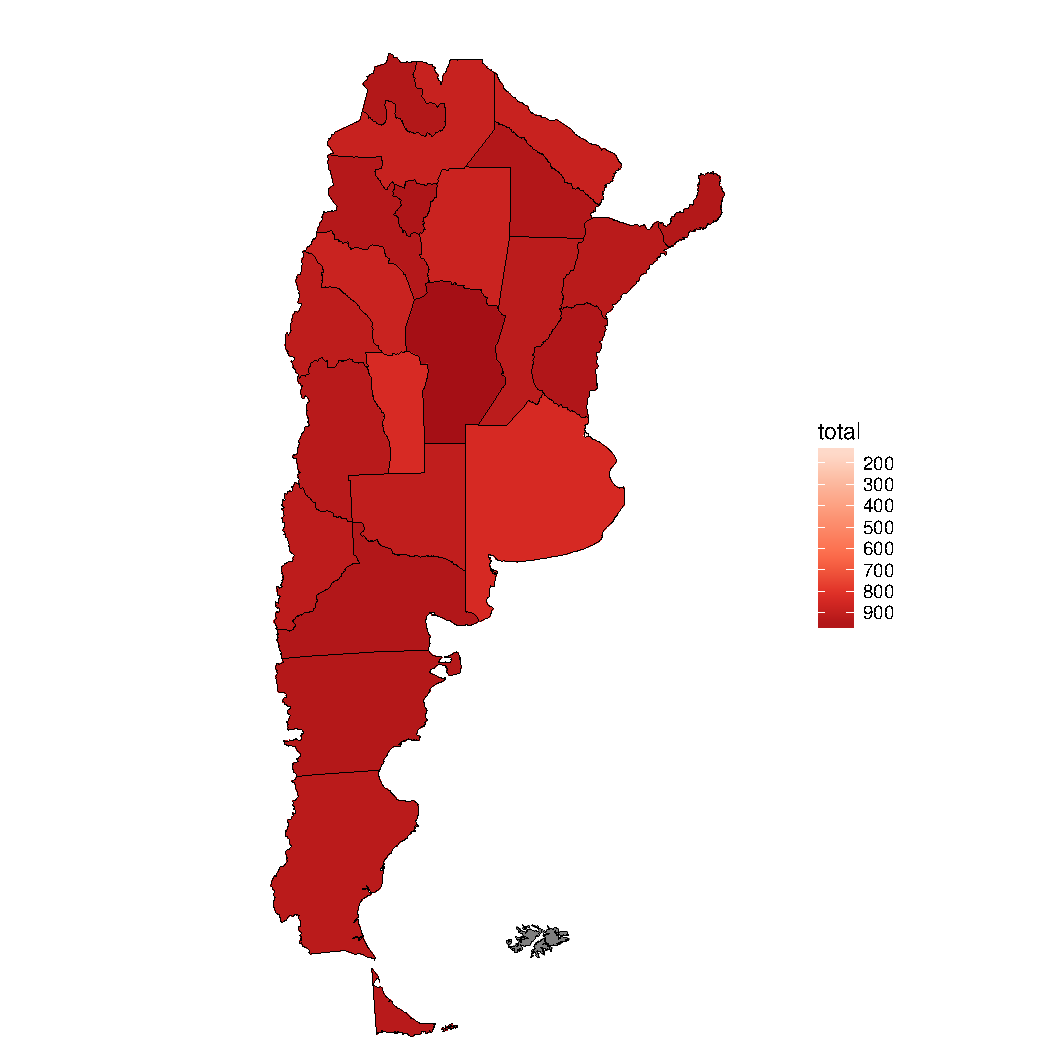
\includegraphics[width=\linewidth]{./images/mapaprovincias.pdf}
    \caption{} 
    \label{fig:mapaProvincias} 
   \end{subfigure}
   \begin{subfigure}[t]{0.31\textwidth}
    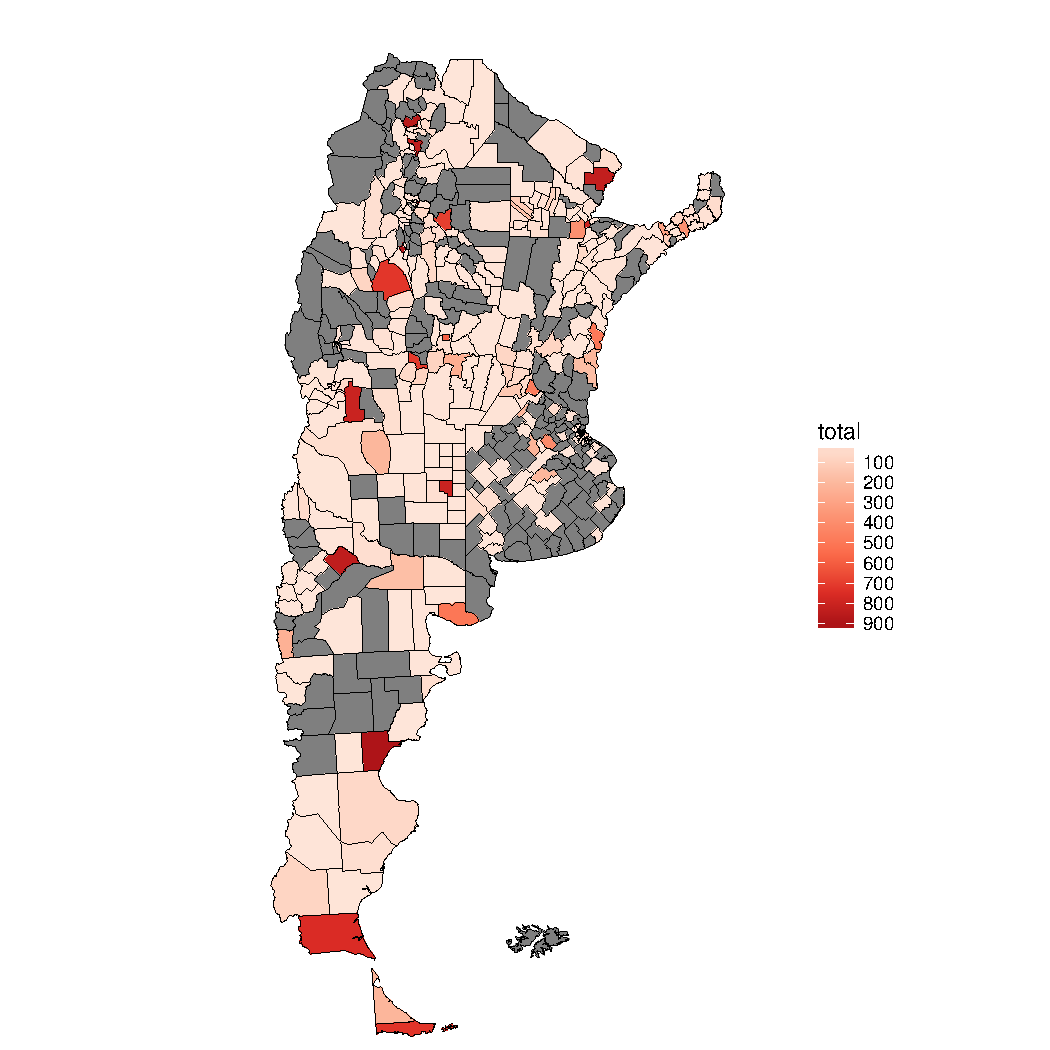
\includegraphics[width=\linewidth]{./images/mapadepartamentos.pdf}
    \caption{} 
    \label{fig:mapaDepartamentos} 
   \end{subfigure}
   \begin{subfigure}[t]{0.31\textwidth}
    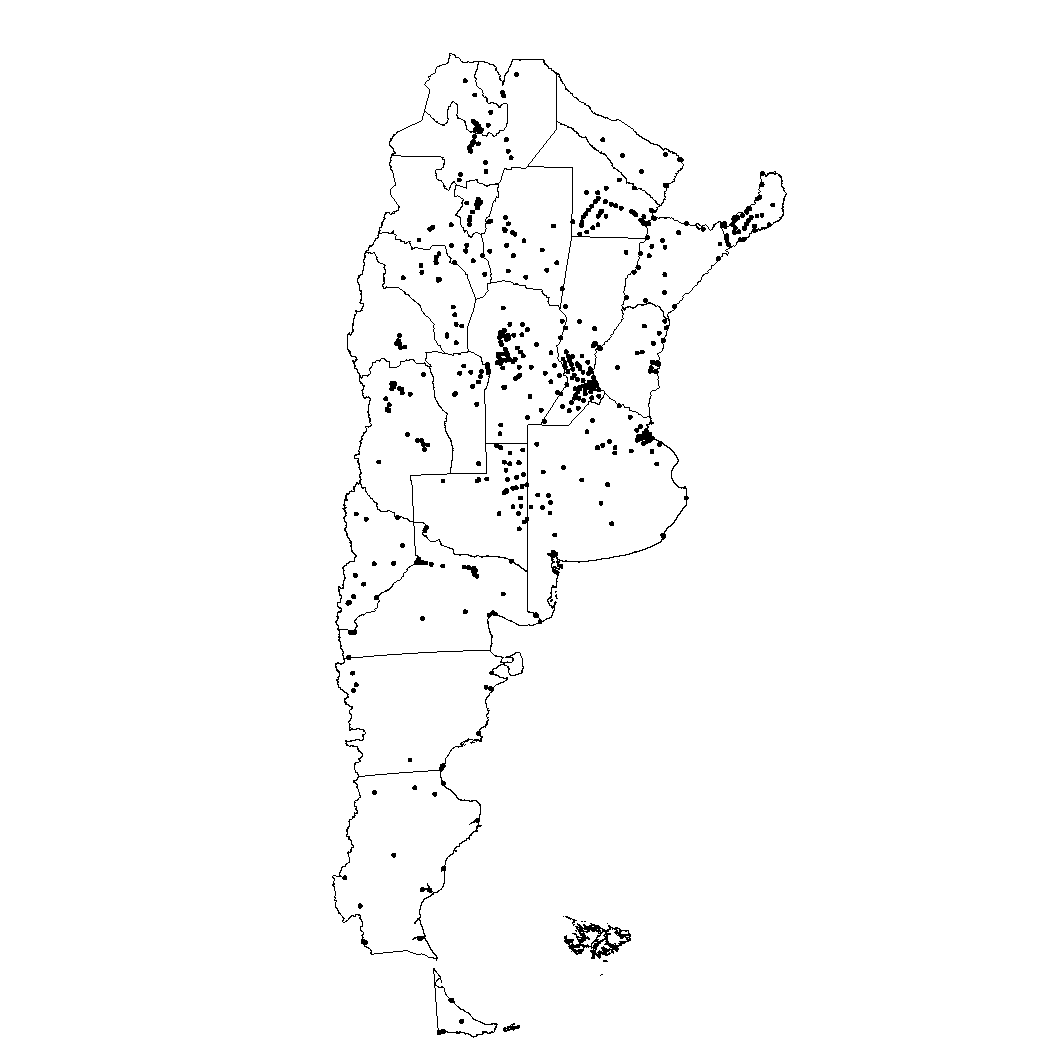
\includegraphics[width=\linewidth]{./images/mapaprovinciasConPuntos.pdf}
    \caption{} 
    \label{fig:mapaPuntos} 
   \end{subfigure}
   



   \caption{Ubicaciones de los usuarios: \subref{fig:mapaProvincias} Mapa de Argentina con la distribución de los usuarios en las provincias sobre el conjunto de desarrollo. \subref{fig:mapaDepartamentos} Distribución de los usuarios en los departamentos sobre el conjunto de desarrollo. Se muestra con áreas grises los departamentos que no poseen usuarios que hayan definido el campo ubicación de su perfil en ese lugar. \subref{fig:mapaPuntos} Distribución de las coordenadas obtenidas a partir de todos los usuarios del conjunto de desarrollo. Las coordenadas fueron obtenidas a través de un proceso de geocodificación. } 
  \label{fig:busqueda_usuarios} 

\end{figure}

En la Figura \ref{fig:mapaProvincias} podemos observar que los usuarios que obtuvimos en las búsquedas se distribuyen de manera uniforme a través de las provincias. Si bien en la Figura \ref{fig:mapaDepartamentos} hay regiones grises que indican la ausencia de usuarios en ese lugar, cabe destacar que los mapas se realizaron obteniendo las coordenadas geográficas a partir de la ubicación definida en el perfil del usuario. Por lo tanto, si una persona declara que vive en \textit{Tucumán, Argentina}, contabilizamos como que esa persona vive en la capital de esa provincia, lo cual puede no ser cierto. Sin embargo, esto no invalida los resultados puesto que la granularidad del análisis es a nivel provincial. Finalmente para ver la distribución de las coordenadas de los usuarios a lo largo del país mostramos la Figura \ref{fig:mapaPuntos}. Se puede observar que en la mayoría de las grandes ciudades hay usuarios en nuestro conjunto de datos. Podemos observar en la Figura \ref{fig:mapaGPS} del apéndice un mapa donde se contabilizaron todos los tuits con coordenadas geográficas del conjunto de datos. En este gráfico se puede observar que la distribución es mucho más amplia, aunque sigue habiendo mayor concentración de usuarios en aquellos departamentos con mayor densidad poblacional.

% \section{Datos de desarrollo y de validación}

% Por cada provincia se tomó a los usuarios de la misma y se los dividió para tener un conjunto de datos de desarrollo y uno de validación. El conjunto de validación fue creado para poder corroborar que los resultados obtenidos por el análisis del conjunto de desarrollo no sean algo intrínseco de esta muestra, sino que se pueden extrapolar a toda la población. 
% La división de los datos se realizó de manera tal que los conjuntos resultantes sean lo más independientes posibles: 
% \begin{description}
%     \item [Usuarios disjuntos] Debido a que ciertos usuarios repiten palabras constantemente, ya sea porque son bots o simplemente porque hablan siempre de los mismos temas, es adecuado validar los resultados con textos producidos por distintos usuarios. De esta manera se intentó mitigar el ruido generado por estos usuarios particulares.
%     \item [Fechas disjuntas] Al analizar los resultados sobre los textos generados en un tiempo acotado de tiempo, estamos trabajando con una muestra específica que es de esperar que tenga fenómenos particulares debido al momento en que fueron escritos. Por ejemplo, debido a cierto fenómeno climático o en el transcurso de un evento polémico (como un debate presidencial o un torneo deportivo), se pueden obtener tuits con una frecuencia de ciertas palabras muy distinta a la frecuencia que tiene normalmente. Por esta razón se dividieron los tuits producidos por los usuarios de manera tal que sus fechas sean disjuntas.
% \end{description}

% La división fue de la siguiente manera:
% Sobre el conjunto de usuarios se dividió en dos de forma aleatoria, con lo que se obtuvo $Usuarios_1$ y $Usuarios_2$. Luego se buscó la fecha $Fecha_{DIV}$ por la cual había una cantidad equiparable entre el conjunto de tuits producidos por  $Usuarios_1$ antes de $Fecha_{DIV}$ y el conjunto de tuits producidos por $Usuarios_2$ después de $Fecha_{DIV}$. Para encontrar la fecha se hizo una búsqueda binaria: dada una fecha $Fecha_{temp}$ (inicialmente es el día intermedio entre la fecha del primer y último tuit recolectado) se calcula la cantidad de tuits que hay con fechas anteriores sobre el conjunto de usuarios $Usuarios_1$ y análogamente se calcula la cantidad de tuits posteriores a esa fecha sobre el otro conjunto de usuarios. Si la cantidad del primer conjunto de tuits es menor que la del segundo conjunto, la $Fecha_{DIV}$ se busca en  el intervalo [$Fecha_{temp}-FechaFinal$] y se repite el procedimiento. Por lo tanto se cumple la siguiente ecuación:

% \begin{equation}
% %\sum_{ f = FechaInicial}^{Fecha_{Div}} tweets(Usuarios_1,f) \approx \sum_{ f = Fecha_{Div}}^{FechaFinal} tweets(Usuarios_2,f) 
%  Fecha_{DIV}  = \operatorname*{arg\,min}_{F} \left|\sum_{ f = FechaInicial}^{F} tuits(Usuarios_1,f) - \sum_{ f = F}^{FechaFinal} tuits(Usuarios_2,f)\right|
% \end{equation}
% Donde $FechaInicial$ es la fecha del primer tuit recolectado  y $FechaFinal$ es la del último.\\

% Después de fijar la fecha se dividió el conjunto de tuits producidos por estos usuarios: el conjunto de desarrollo con los tuits producidos antes de $Fecha_{DIV}$ y el conjunto de test producidos posteriormente a esa fecha.

\section{Tokenización y normalización}

En cuanto al análisis del texto surge una primer problemática: ¿qué es una palabra? En principio podemos definir a una palabra como cualquier secuencia de caracteres delimitados por espacios blancos. Con esta definición \textit{523456} y \textit{?} serían palabras. Debido a esto podríamos restringir nuestra definición a una secuencia de caracteres alfabéticos. Los ejemplos mencionados anteriormente dejarían de estar dentro de la definición. Sin embargo términos como \textit{asdsdafsdf} también serían palabras. Para evitar este problema podríamos tener un diccionario como filtro para saber si una secuencia de caracteres dada es una palabra. Si bien esto tendría mucha precisión al momento de filtrar los términos, no sería capaz de detectar palabras que existen en una lengua pero que no están incluidos en el diccionario elegido. Además, dada la cantidad de palabras recogidas, es altamente improbable que una secuencia al azar de caracteres alfabéticos reúna las condiciones de frecuencia necesarias para resultar destacada por la métrica que utilizamos. Es por eso que decidimos tomar a una palabra como una secuencia de caracteres alfabéticos.

Es muy posible que tengamos palabras que no sean interesantes a nivel lingüístico, como errores de tipeo (e.g. computadira, escribur), errores ortográficos o  nombres propios. Es importante destacar que Twitter tiene caracteres especiales para mencionar a la gente, como el @, o el \#(hashtag) utilizado para agrupar mensajes. Estos caracteres aparecen mucho, ya que los usuarios suelen responderse en la red, mencionando los mismos temas (aclarando el hashtag), o respondiendo a otros usuarios. Ya que esos caracteres no son alfabéticos, cualquier término que los utilice no va a ser parte del conjunto de palabras, como tampoco lo serán las direcciones de páginas web. Decidimos ignorar estos términos ya que no tienen interés lingüístico y agregarían mucho ruido a los datos.

Además de la tokenización, se realizó una normalización del texto. Todas las letras se convirtieron a letra minúscula y las palabras con más de tres letras iguales de forma consecutiva se redujeron para que solo tengan tres repeticiones. De esta forma, el término \textit{padreeeee} y \textit{padreeee} fueron reducidos a una única unidad léxica (\textit{padreee}). Esto se hizo con la librería \textit{TweetTokenizer de NLTK}. 
Como ya dijimos, se descartó la idea de filtrar las palabras que no estuvieran en un diccionario ya que si bien hubiera eliminado mucho ruido, también nos hubiera filtrado palabras de interés. Este es el caso de los neologismos, o las palabras que, si bien se utilizan hace mucho tiempo, no están en los diccionarios actuales.

\section{Caracterización de la muestra}

Para tener una noción más completa de la muestra, se presenta la Tabla \ref{tab:cantidades}, que indica las cantidades de palabras y tuits por provincia. Puede notarse que la muestra está balanceada con respecto a la cantidad de usuarios, tuits por provincia y palabras. Los tuits realizados en la Ciudad Autónoma de Buenos Aires están incluídos en los de la provincia de Buenos Aires. Tomamos esta decisión ya que debido al constante movimiento entre las personas de la ciudad y la provincia, es difícil distinguir de forma fehaciente a los usuarios de ambos territorios.


\begin{table}[ht]
\centering


\begin{tabular}[width=0.7\textwidth]{|l|c|c|c|c|c|c|}
\hline
Provincia      & \#Palabras Distintas & \#Usuarios & \#Tuits & \#Total Palabras \\ \hline
Buenos Aires   & 191919       & 920          & 1125042    & 8974372  \\
Catamarca      & 173104       & 957          & 1057019    & 8161309   \\
Chaco          & 169476       & 964          & 976943     & 7605991   \\
Chubut         & 182592       & 954          & 1023373    & 8884745   \\
Córdoba        & 207307       & 987          & 1224266    & 10075932  \\
Corrientes     & 183292       & 939          & 1044951    & 8426940   \\
Entre Ríos     & 188679       & 969          & 1193693    & 9462986  \\
Formosa        & 169254       & 903          & 923352     & 7184382   \\
Jujuy          & 171064       & 971          & 678004     & 5951778   \\
La Pampa       & 186593       & 935          & 1085757    & 8996318  \\
La Rioja       & 186041       & 946          & 704044     & 6757277  \\
Mendoza        & 193708       & 945          & 1099717    & 9402399   \\
Misiones       & 168400       & 972          & 984218     & 7790197   \\
Neuquén        & 188038       & 927          & 1111201    & 9021449   \\
Río Negro      & 194383       & 965          & 1215361    & 9991831  \\
Salta          & 188402       & 884          & 830916     & 7506652   \\
San Juan       & 183546       & 926          & 1002322    & 8377792  \\
San Luis       & 164185       & 896          & 1006464    & 8327093  \\
Santa Cruz     & 174089       & 935          & 876621     & 7432923  \\
Santa Fe       & 201879       & 937          & 1019620    & 8862328  \\
Santiago del Estero       & 166540       & 887          & 944109     & 7355729  \\
Tierra del Fuego & 197273       & 964          & 976426     & 8559218   \\
Tucumán        & 195643       & 962          & 1093874    & 9238526 \\
  \hline
\end{tabular}
\caption{Cantidades del conjunto de datos}
\label{tab:cantidades}
\end{table}



También analizamos la cantidad de palabras por tuit promediadas sobre cada usuario.
Debido a que los tuits están limitados a 140 caracteres, era de esperar que no hubieran demasiadas palabras promedio por cada tuit. En la Figura \ref{fig:cantPalabrasUsuario} podemos observar que la media para la cantidad de palabras promedio en un tuit está entre 7 y 8.
\begin{figure}[!ht]\centering
  \begin{subfigure}[t]{0.49\textwidth}
    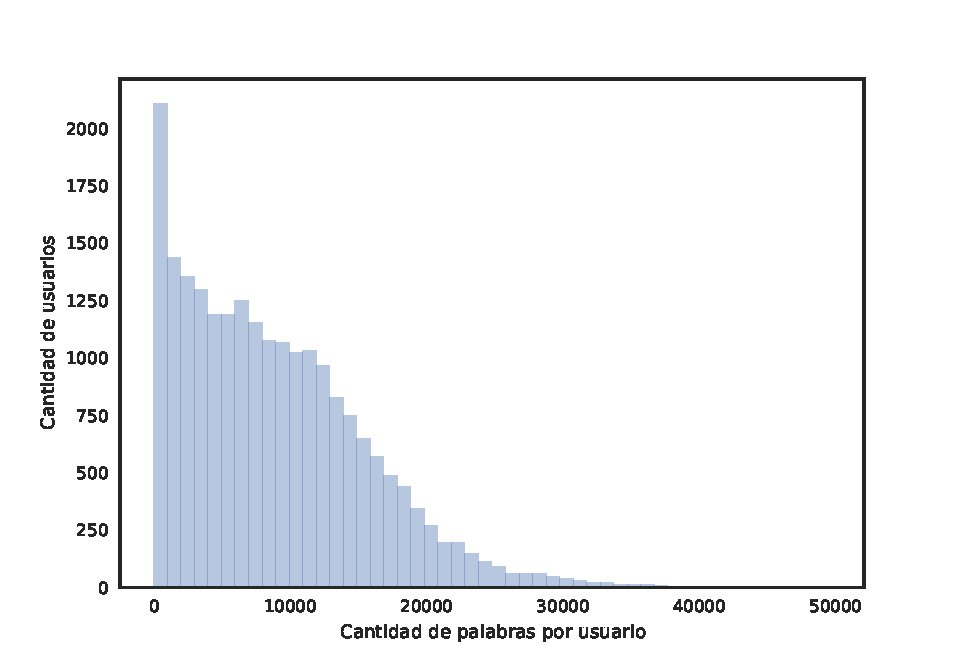
\includegraphics[width=\linewidth]{images2/cantPalabrasUsuario_sinFiltro.pdf}
    \caption{} 
    \label{fig:cantPalabrasUsuario} 
   \end{subfigure}
   \begin{subfigure}[t]{0.49\textwidth}
    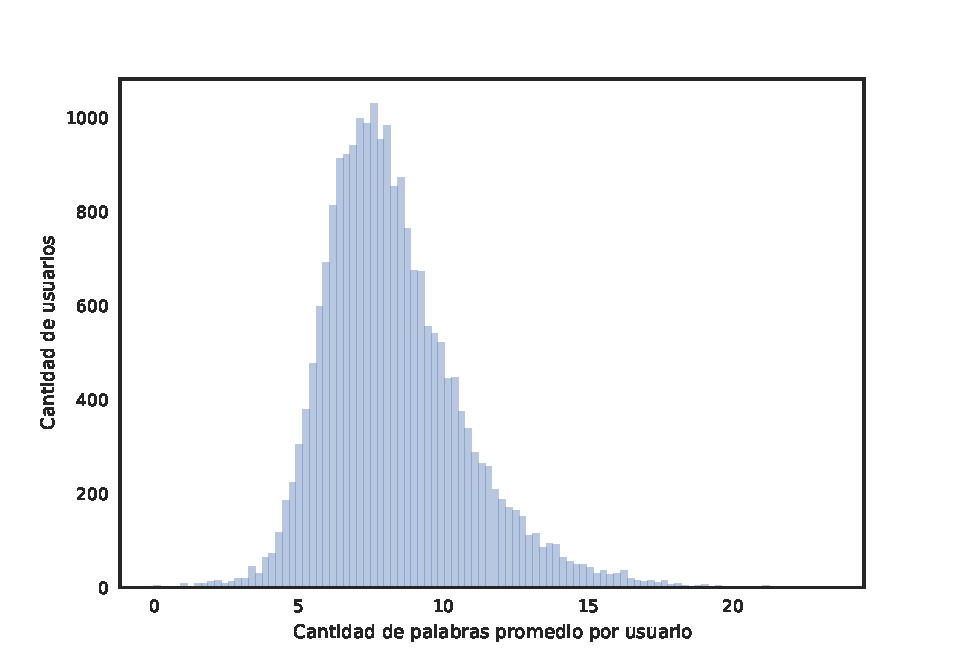
\includegraphics[width=\linewidth]{images2/cantPalabrasPromedio_sinFiltro.pdf}
    \caption{} 
    \label{fig:cantPalabrasPromedio} 
   \end{subfigure}
   \caption{ Histogramas: \subref{fig:cantPalabrasUsuario} Cantidad de palabras totales por usuario. \subref{fig:cantPalabrasPromedio} Cantidad de palabras en promedio por tuit, para todos los usuarios.}
\end{figure}

%Cantidad de palabras promedio por tweet
%Cantidad de palabras por usuario + varianza por provincia
\subsection{Distribución temporal de tuits}
Los tuits recolectados para el conjunto de datos de desarrollo tienen una particularidad: la cantidad de tuits recolectados crece año a año. Esto se refleja en los gráficos de la Figura \ref{fig:histTweets}, que muestran la progresión temporal de la cantidad de tuits en cuatro regiones representativas: La Pampa, Buenos Aires, Chaco y Neuquén.

\begin{figure}[!ht]\centering
   \begin{subfigure}[t]{0.49\textwidth}
     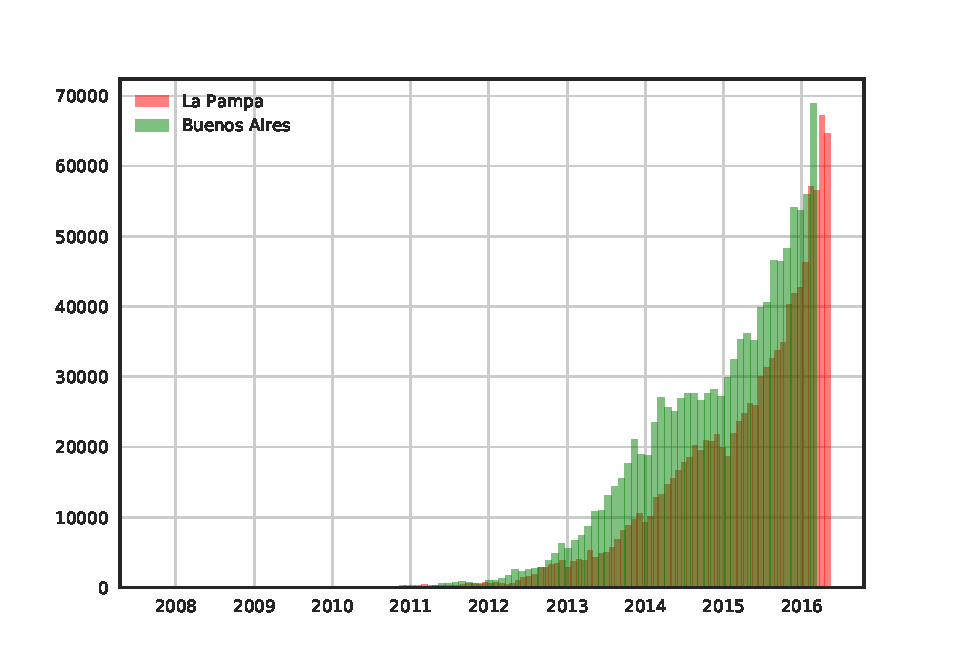
\includegraphics[width=\linewidth]{images2/histTweetsProvincia1_sinFiltro.pdf}
     \caption{}
     \label{fig:histTweetsProvincia1}
   \end{subfigure}
   \begin{subfigure}[t]{0.49\textwidth}
     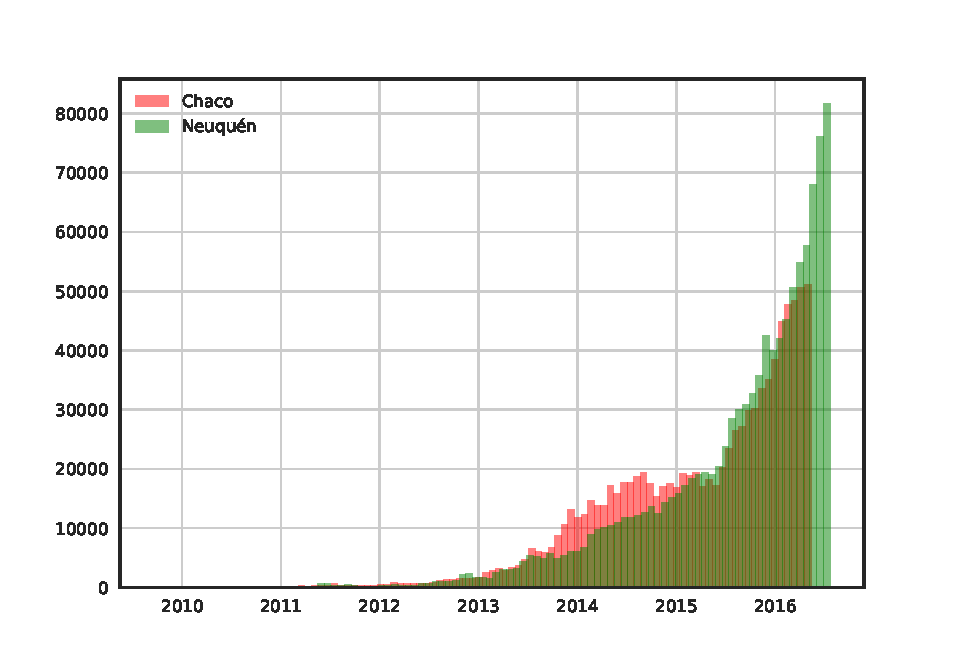
\includegraphics[width=\linewidth]{images2/histTweetsProvincia2_sinFiltro.pdf}
     \caption{}
     \label{fig:histTweetsProvincia2}
   \end{subfigure}
   \caption { \subref{fig:histTweetsProvincia1} Histograma de la cantidad de tuits que se hicieron por intervalo de tiempo en la provincias La Pampa y Buenos Aires. \subref{fig:histTweetsProvincia2} Gráfico para Chaco y Neuquén.}
   \label{fig:histTweets}
\end{figure}


% Tweets promedio por usuario, por provincia. (varianza)

% cantidad de tweets por usuario, cantidad media de palabras por usuario

\section{Métricas para detectar léxico contrastivo}
\section{Búsqueda de contrastes}

% Definir que es un contraste, que tiene un uso significativo en una region más que en otra. LAs alternativas que propusimos, z test binomial.
Una palabra tiene un contraste cuando esta tiene un uso con diferencias significativas en
distintas regiones. En este trabajo nos propusimos crear un listado con palabras con contrastes que tengan
importancia a nivel lingüístico. En este sentido, los nombres de personas, lugares u organizaciones no 
fueron considerados de interés a pesar de tener contrastes en su uso.
Este listado fue ordenado por una métrica que capte en un único valor el nivel contrastivo. De esta manera, 
se seleccionó un subconjunto de palabras, de acuerdo a la métrica, el cual fue analizado manualmente en otros textos por la Academia Argentina de Letras.

El primer acercamiento para ver el contraste de las palabras lo realizamos comparando las frecuencias de las palabras 
en cada par de provincias de la Argentina. Para esto calculamos, por cada palabra, la frecuencia de ocurrencias sobre cada una de las dos provincias. La mayor frecuencia de ambas, la llamamos frecuencia máxima y a la menor, la frecuencia mínima. Luego el cociente entre la frecuencia máxima y la frecuencia mínima tiene como resultado lo que llamamos \textit{maxDif}. En caso de que en una de las dos provincias no se haya 
recolectado tuits con esa palabra, se tomaba como frecuencia mínima a la frecuencia mínima distinta de 0 de todas las palabras generadas en esa provincia. Así se evitó la división por cero. Esta métrica se resumen en la ecuación \ref{eq:maxDif}.


\begin{equation}
  \label{eq:maxDif} 
  maxDif(w,p_1,p_2) = \frac{F_{max}(w,p_1,p_2)}{F_{Min}(w,p_1,p_2)}
\end{equation}
donde 
\begin{equation}
F_{max}(w) = \max(frec(w,p_1),frec(w,p_2))
\end{equation}

%TODO: arreglar el overfull OK
\begin{equation}
 F_{min}(w) = \left\{ \begin{array}{ll}
             \min(frec(w,p_1),frec(w,p_2))  \text{ si } frec(w,p_1) * frec(w,p_2) > 0  & \\
             \\
             \min(frec(w,p))  \forall w \in palabras(p) , \text{ con } p=\{p_1,p_2\} \setminus \{P_{max}\} \text{sino} &  \\
             \end{array}
   \right.
\end{equation}
   donde $P_{max}$ es la provincia que tiene la mayor frecuencia de ambas.



De esa manera se ordenó el listado de cada par de provincias teniendo en cuenta la división de frecuencias. 
Sin embargo, este método imposibilitaba el trabajo manual para la Academia Argentina de Letras que debía mirar estos listados y hacer un análisis más exhaustivo sobre las palabras con mayor diferencia de frecuencias, debido a que había $\binom{23}{2} = 253$
listados (o equivalentemente 253 columnas en un mismo listado) a analizar. Además la métrica solo permitía saber si había un contraste entre dos provincias, pero no se podía tener en cuenta la frecuencia de la palabra en el resto de las provincias. 
% Mencionar que la idea era realizar un z test para obtener las palabras más significativas.
En consecuencia las palabras se encontraban repetidas en los distintos listados y con diferentes valores de \textit{maxDif}, lo cual hacía muy difícil poder identificar en que regiones había una diferencia significativa de frecuencias.
Debido a esto decidimos realizar un nuevo enfoque para encontrar las palabras con alta contrastividad en las distintas regiones, de manera que una métrica pueda reflejar el nivel de contrastividad de la palabra en un único valor. En primer lugar intentamos modificar la métrica \textit{maxDif} de la siguiente manera: 
Sea $f_{max}(w)$ la frecuencia máxima entre las frecuencias de todas las provincias y sea $f_{min}$ la frecuencia mínima distinta de $0$ sobre todas las provincias, luego la métrica generalizada \textit{$maxDif_g$} se puede definir como

\begin{equation}
 maxDif_g(w) = \frac{f_{max}(w)}{f_{min}(w)}
 \label{eq:maxDifg}  
\end{equation} 

Si bien esta métrica logra resumir en un único valor la diferencia de frecuencias, sigue sin considerar la dispersión de las frecuencias en todas las provincias.
Por este motivo, nos enfocamos en analizar el contraste de frecuencias de palabras sobre las provincias a través de una métrica superadora.

\subsection{Métricas para medir el contraste en la frecuencia de las palabras}
Dado que se quieren encontrar las palabras con contrastes significativos en distintas 
regiones se propone generar una métrica basada en la cantidad de información 
para poder realizar esta tarea.

Una medida que se puede usar para comparar las frecuencias de las palabras en las diferentes regiones del país puede ser la entropía definida por Shannon ( ver en el apéndice: \ref{sub:entropiaShannon}), debido a que nos brinda un valor que informe qué tan uniforme es la distribución de las frecuencias de cada palabra. La entropía es máxima cuando la probabilidad de los eventos es equiprobable y mínima en el caso que la probabilidad de un evento es 1.
Sin embargo, la entropía como única medida tiene sus desventajas. En particular, una palabra con una sola ocurrencia en una provincia y ninguna en las demás, tiene la entropía mínima. A pesar de que nos interesan las palabras con un contraste significativo entre regiones, dentro de ellas elegiremos las que tienen mayor cantidad de ocurrencias. Es por esto que elaboramos otra métrica que tenga en cuenta la entropía, entre otras variables a tener en cuenta.


\subsection{Valor de información}
La métrica que utilizamos para ordenar los listados de palabras y detectar cuáles son
las que tienen altos contrastes en su uso en distintas regiones fue inspirada por el
trabajo de Zanette y Montemurro \cite{montemurro2010towards}.
Ellos, a diferencia de Shannon, estudiaron una relación entre una medida de la información y su función semántica en el lenguaje.
A continuación detallamos el procedimiento para calcular lo que los autores llamaron
el valor de la información:

Dado un texto dividido en $P$ partes iguales llamadas ventanas, se calcula la entropía  $H(w)$ sobre el vector de cantidad de ocurrencias en cada una de las $P$ ventanas.
Luego se define $\widehat{H(w)}$  como la entropía de una permutación aleatoria del texto y promediada por todos las posibles realizaciones de la permutación de él. 
%% TODO: CHEQUEAR LA DEFINICION DE LA ENTROPIA SHUFFLEADA

Es decir, se distribuyen uniformemente las palabras en $P$ partes y se calcula la
entropía como se hizo con el texto original. Es de esperar que en la mayoría de casos 
la entropía del texto permutado sea mayor que la medida en el calculo original. Esto 
se debe a que las palabras se distribuyen de forma más uniforme 
en las distintas partes.

Finalmente, definen al valor de la información como $I(w) = p(w) (\widehat{H(w)} - H(w))$, con $p(w)$ la frecuencia total de la palabra en el texto. 
De esta manera se les da más importancia a las palabras que son más frecuentes y a las palabras que tienen una baja entropía, ya que en estas el término de la diferencia es más grande.

Zanette et al. analizaron el valor de la información sobre tres textos, \textit{Análisis de la mente}, 
\textit{Moby Dick} y \textit{El origen de las especies} de Charles Darwin. 
En los tres libros las palabras con mayor valor de la información están 
altamente relacionadas con los temas principales.

Si bien esta métrica tiene en cuenta la frecuencia de las palabras además de la 
entropía, el texto en Twitter resulta difícil de dividir en partes iguales. 
Esto es porque la división está pensada para dividir el texto en secciones que 
posiblemente hablen de distintos temas y nuestros textos son tuits que por lo general no superan las 10 palabras.
Otra dificultad que surge de esta métrica es la imposibilidad de realizar la media 
de todas las posibles permutaciones del texto por la limitación computacional ya que 
tenemos una cantidad muy grande de datos. Es por eso que diseñamos una métrica similar basada en una aproximación de la entropía máxima de una palabra.

Podemos pensar a las palabras del texto como una variable aleatoria $W$, donde cada palabra $w$ tiene una probabilidad de aparición en una provincia dada de la Argentina. Esta probabilidad la aproximamos con la frecuencia en la que aparece, es decir la cantidad de ocurrencias de la palabra dividida por la cantidad de palabras totales.
Por otro lado sea $P$ una variable aleatoria que cuenta la cantidad de personas que 
utilizan la palabra $p$ en cada provincia.

\medskip

Luego, sea $cant_w(p)$ igual al logaritmo sobre la cantidad de ocurrencias de esa palabra en toda la Argentina, es decir $cant_w(p) = \log_2(cantidadOcurrencias(p))$ .y sean las constantes $MIN_w$ y $MAX_w$ definidas de la siguiente manera:


% \noindent\begin{minipage}{.5\linewidth}
% \begin{equation}
% MIN_W = \min\limits_{p \in Palabras} cant_w(w)
% \end{equation}
% \end{minipage}%
% \begin{minipage}{.5\linewidth}
% \begin{equation}
%   MAX_W = \max\limits_{p \in Palabras} cant_w(w)
% \end{equation}
% \end{minipage}

\begin{equation}
MIN_W = \min\limits_{p \in Palabras} cant_w(w)
\end{equation}

\begin{equation}
  MAX_W = \max\limits_{p \in Palabras} cant_w(w)
\end{equation}

Realizamos una normalización lineal de la función $cant_w$, 

\begin{equation}
norm_{w}(p) = \frac{cant_w(p)- MIN_W }{MAX_W - MIN_W}
\label{eq:norm1}
\end{equation}

De esta manera, $norm_w$ tiene su imagen en el rango $[0,1]$, tomando el valor $0$ sobre la palabra que tiene la cantidad de ocurrencias máxima y toma el valor $1$ cuando se aplica a la palabra con menor cantidad de ocurrencias. Vale la pena aclarar, que tomamos $40$ como umbral mínimo de cantidad de ocurrencias de las palabras para ser estudiadas.
A partir de la función $norm_w$ definimos el valor de la información de las palabras $I_w$ como:

\begin{equation}
I_w(w) = norm_{w}(w) * (\widehat{H}_{w}(w) - H_{w}(w)) \\
\label{eq:iw}
\end{equation}

siendo $H_w(w)$ la función de entropía calculada sobre las cantidades de ocurrencias de la palabra $w$ sobre las 23 provincias argentinas. De forma similar $\widehat{H}$ es la función de entropía sobre las cantidades de ocurrencias simuladas en todas las provincias a partir de una distribución multinomial. Elegimos esta distribución ya que con esta se distribuye la suma de los valores de la variable aleatoria, en nuestro caso la cantidad de ocurrencias de la palabra $w$, de forma uniforme.%TODO: explicar más en detalle

Ahora bien, una determinada provincia o región pueden tener muchas ocurrencias de una palabra formuladas por algunos pocos usuarios que utilizan constantemente el término. Un ejemplo de esto podrían ser bots que escriben automáticamente textos iguales (o similares) en grandes cantidades. Otra posible causa de este fenómeno podría ser la de usuarios que hablan de personas, lugares o marcas de forma constante.
Es por esto que realizamos una métrica similar que tenga en cuenta la diferencia de la entropía sobre la cantidad de personas que utilizan la palabra . Agregandole el término $norm_u$, que es la constante normalizadora de la cantidad de usuarios descripta en la ecuación \ref{eq:norm2} obtenemos el valor de la información de las personas $I_u$,

\begin{equation}
I_u(w) = norm_{u}(w) * (\widehat{H}_{u}(u) - H_{u}(w))
\label{eq:iu}
\end{equation}

Donde,
\begin{equation}
norm_{u}(w) = \frac{cant_u(w)- MIN_U }{MAX_U - MIN_U}
\label{eq:norm2}
\end{equation}
\begin{equation}
 MIN_U = \min\limits_{p \in Palabras} cant_u(p)
\end{equation}
\begin{equation}
  MAX_U = \max\limits_{p \in Palabras} cant_u(p)
\end{equation}

y $cant_u(p)$ es el logaritmo sobre  la cantidad de usuarios que utilizan dicha palabra en la Argentina, es decir $cant_u(p)= \log_2(cantidadUsuarios(p)))$.

Debido a que queremos tener en cuenta tanto a la variación de la cantidad de ocurrencias de la palabra como a la variación de la cantidad de usuarios, elegimos como métrica la multiplicación de ambas métricas definidas, es decir  

\begin{equation}
%I(w) =  norm_{p}(w) * norm_{u}(w) * (\widehat{H}_{w}(w) - H_{w}(w)) * (\widehat{H}_{p}(w) - H_{p}(w)) \\
I(w) =  I_w(w) * I_u(w)\\
\label{eq:ivalor}
\end{equation}

Es importante aclarar que tanto $norm_{w}$ como $norm_{u}$ realizan una normalización del logaritmo de esas variables. Esto se debe a que el logaritmo genera una dispersión tal que agrupa los valores altos que se encontraban muy dispersos mientras que separa los valores pequeños que estaban concentrados. Esto se puede ver en las figuras \ref{fig:cantNormUsuarios} y \ref{fig:cantNormPalabras}.


%TODO: ejemplificar la variacion de la entropia.  La variacion de la entropia se puede ver como una cantidad que mide cuanta información se necesita para poder obtener esa distribución
% Si las cantidades de ocurrencias (o de personas que utilizan) de un término están distribuidas uniformemente a través de todas las provincias, quiere decir que no aporta demasiada información 

\begin{figure}[!ht]\centering
  \begin{subfigure}[t]{0.49\textwidth}
    \includegraphics[width=\linewidth]{./images/DistribucionOcurrenciasPalabrasAnotaciones.pdf}
    \caption{}
    \label{fig:cantPalabras} 
   \end{subfigure}
   \begin{subfigure}[t]{0.49\textwidth}
    \includegraphics[width=\linewidth]{images2/cantUsuarios_sinFiltro.pdf}
    \caption{}
    \label{fig:cantPalabrasPromedio} 
   \end{subfigure}
   \caption{La figura \ref{fig:cantPalabras} muestra un histograma de la cantidad de ocurrencias de las palabras. En la figura \ref{fig:cantPalabrasPromedio} se puede observar un histograma de la cantidad de usuarios que utilizan una determinada cantidad de palabras.}  
\end{figure}

Para eliminar los valores atípicos se procedió a remover tanto las palabras que no superaran las 40 ocurrencias, como también aquellas que eran dichas por menos de 6 usuarios. La métrica se evaluó en este conjunto filtrado de palabras. 

\subsection{Frecuencia de las palabras}
\label{sub: frecuenciaPalabras}
% Ver si se hace este gráfico con todas las palabras ya que por ahora tengo el conjunto de palabras con más de 40 ocurrencias
En la figura \ref{fig:cantPalabras} graficamos la distribución de la cantidad de ocurrencias de las palabras. Podemos observar que la mayoría de las palabras ocurren poco. En particular el 50\% de las palabras ocurren menos de 139 veces. Por otro lado hay pocas palabras que ocurren mucho, por ejemplo la palabra \textit{que} o la preposición \textit{de}.


\begin{figure}[!ht]\centering
  \begin{subfigure}[t]{0.49\textwidth}
    \includegraphics[width=\linewidth]{./images2/cantNormUsuarios_sinFiltro.pdf}
    \caption{} 
    \label{fig:cantNormUsuarios} 
   \end{subfigure}
   \begin{subfigure}[t]{0.49\textwidth}
    \includegraphics[width=\linewidth]{images2/cantNormPalabras_sinFiltro.pdf}
    \caption{} 
    \label{fig:cantNormPalabras} 
   \end{subfigure}
   \caption{La figura \ref{fig:cantNormUsuarios} muestra un histograma de la normalización de la cantidad de ocurrencias de las palabras, definida como $norm_u$. La figura \ref{fig:cantNormPalabras} contiene un histograma de la normalización sobre la cantidad de usuarios que utilizan una determinada cantidad de palabras definida como $norm_w$.}
\end{figure}


\begin{table}[ht]
\centering
\label{tab:palabrasMasOcurrentes}
\begin{tabular}{ c c }
\toprule
Palabra & Cantidad de Ocurrencias \\ 
\midrule
que     & 7509160                 \\
de      & 6527014                 \\
a       & 4962492                 \\
la      & 4913854                 \\
no      & 4177810                 \\
me      & 4101998                 \\
y       & 3838370                 \\
el      & 3773455                 \\
en      & 2969783                 \\
te      & 2060662                 \\
se      & 1976027                 \\
un      & 1863075                 \\
es      & 1825892                 \\
con     & 1799979                 \\
lo      & 1712189                 \\
mi      & 1643777                 \\
por     & 1553382                 \\
los     & 1498941                 \\
para    & 1398757                 \\
las     & 1212452                 \\
\bottomrule
\end{tabular}
\caption{Cantidad de apariciones de las 20 palabras más frecuentes.}

\end{table}

Si comparamos la posición de la palabra en un listado ordenado podemos ver que  las cantidades de ocurrencias parecieran seguir una distribución zipfiana. La ley de Zipf es una ley empírica formulada por George Zipf en el año 1932 en la cual se establece una relación entre la frecuencia de una palabra con su posición dentro del listado de palabras ordenadas por frecuencia decreciente \cite{montemurro2001beyond,zipf2016human}. En particular, sea $n$ la posición de la palabra en el listado ordenado y sea $f(n)$ la cantidad de ocurrencias de la n-ésima palabra, se puede hacer la siguiente aproximación:

$$f(n) \approx \frac{A}{n^{\alpha}}$$
donde $\alpha$ toma un valor levemente mayor a 1 y $A$ es una constante normalizadora.
Entonces, bajo la ley de Zipf uno puede saber que la frecuencia de la segunda palabra más dicha en un corpus, es aproximadamente la mitad que la primera. La palabra con posición 3 en el listado ordenado por frecuencias, va a tener aproximadamente la tercera parte de la cantidad de ocurrencias que la primera y así sucesivamente. De esta manera hay una relación lineal entre el logaritmo de la posición del listado ordenado por frecuencias y el logaritmo de la cantidad de ocurrencias de cada palabra.
% TODO: escribirlo en ecuación,
Otra forma de utilizar esta ley empírica es la siguiente:
sabiendo la posición de una palabra \textit{w} en el listado ordenado por frecuencias de un corpus \textbf{A} y sabiendo la cantidad de palabras totales de un corpus \textbf{B}, puede estimarse la cantidad de ocurrencias de \textit{w} en el corpus \textbf{B}.
%TODO: HACER EJEMPLO de calculo de frecuencias a traves de la frecuencia de nuestro corpus
%TODO: chequar ecuación de ley de zipf

\begin{figure}[!ht]
\centering
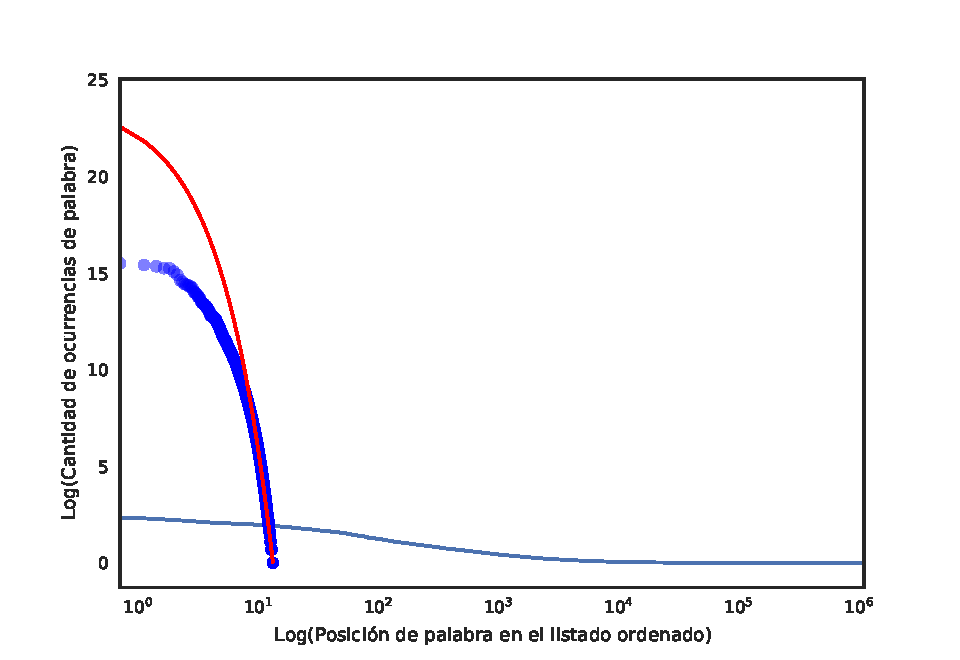
\includegraphics[width=0.5\textwidth]{images2/zipf_sinFiltro.pdf}
\caption{Cantidad de Ocurrencias de palabra vs posición en listado ordenado. Se aplicó el logaritmo natural a las cantidades de ocurrencias, como también a los valores de las posiciones para mostrar la proporcionalidad entre $f(n)$ y $\frac{1}{n^{\alpha}}$.} 
\label{fig:zipf} 
\end{figure}



%Qué resultados obtuvimos del análisis en cuestión. Acá vamos a poner qué palabras fueron significativas, dónde lo fueron, y demás.

% Distribucion de entropía vs frecuencia  
% Distribucion de frecuencias de las palabras
% Distr entropia
% de valor de la inf. a partir de los 5000 se ve que se estanca (graficar hasta 10**5)

% subsection de la region de las palabras --> muestro tabla
% se muestra que las regiones son contiguas geograficamente (hablarlo con santiago)

% Las palabras que se vieron, las primeras generalmente se refieren a lugares o gentilicios



% ver los graficos que hace zanette en su paper

% se busco el dataset de localidades para filtrar las palabras que son lugares

\section{Distribución de la entropía}
Teniendo el listado de palabras hicimos un cálculo de entropía tomando en cada provincia la cantidad de ocurrencias de cada palabra. En la figura \ref{fig:entropiaPalabras} podemos observar la distribución del valor de la entropía sobre todas las cantidades de ocurrencias de las palabras con más de 40 apariciones y dichas por más de 5 usuarios. 

Podemos ver que la mayor parte de las palabras tienen un valor de entropía entre 2.5 y 3. Esto quiere decir que hay un gran conjunto de palabras que tiene una cantidad de ocurrencias relativamente uniforme a lo largo de todas las provincias. Sin embargo, hay otro conjunto de palabras que tienen una entropía menor a 2, la cual podemos considerar como baja. Estas últimas palabras serán las que tienen mayor interés debido a que tienen una variación marcada en cuanto a su utilización en las distintas regiones. El máximo valor alcanzado de la entropía es de $3.1350$ con la palabra \textit{el}. Como aclaración la entropía calculada se realizó con logaritmos naturales, por lo tanto el máximo valor posible es de  $ln(23) = 3.1355$ donde habría una distribución uniforme en la cantidad de ocurrencias sobre las 23 provincias argentinas.

Tener en cuenta únicamente a la entropía de las palabras nos puede generar la detección de palabras que no son de interés, ya sea porque no ocurren una cantidad significativa de veces o porque la variación de las ocurrencias en las distintas provincias se debe solamente a pocos usuarios que la utilizan mucho. Es por esto que también se calculó la entropía teniendo como variable la cantidad de personas que utilizaron cierto término en una determinada provincia.


\begin{figure}[ht]
\centering
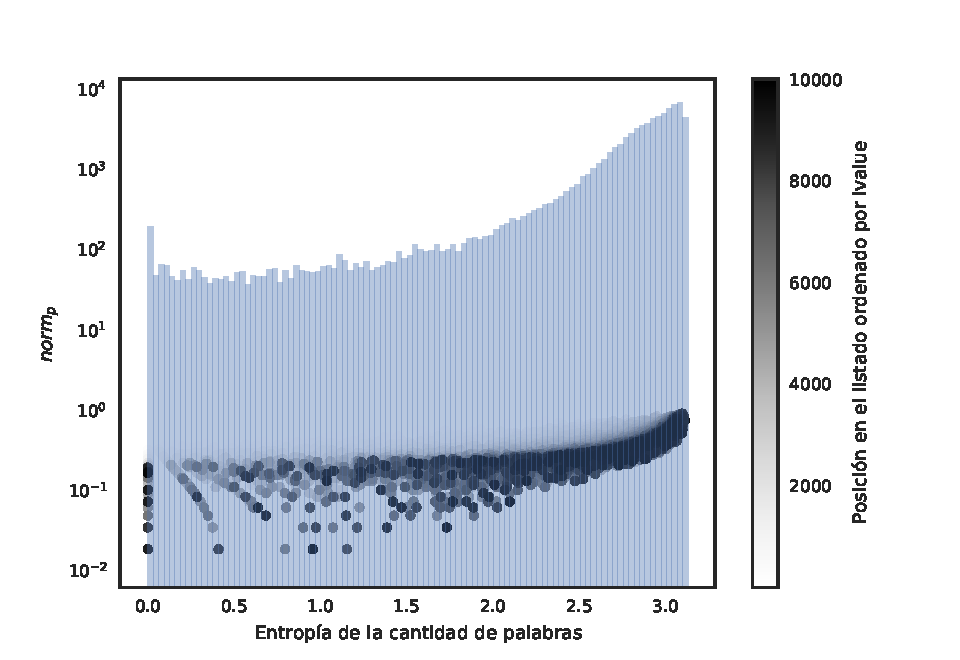
\includegraphics[width=1.0\textwidth]{./images/DistribucionEntropia.pdf}
\caption{Histograma del valor de la entropía de las palabras ($H_w$).} 
\label{fig:entropiaPalabras} 
\end{figure}



\section{Distribución del valor de la información}
\label{sec:ValorDeLaInformacion}
En el gráfico \ref{fig:infoValue} se muestra una clara relación entre la cantidad de ocurrencias que tiene una palabra y su valor de la información, indicado por el color: cuanto más oscuro más alto el valor. A su vez, se nota que el valor de la información suele ser mayor a medida que el valor de la entropía es menor. Esto no siempre es el caso debido a que hay palabras que tiene una entropía de palabras baja, pero sin embargo la entropía de personas es alta logrando que el valor de la información sea bajo.

\begin{figure}[ht]
\centering
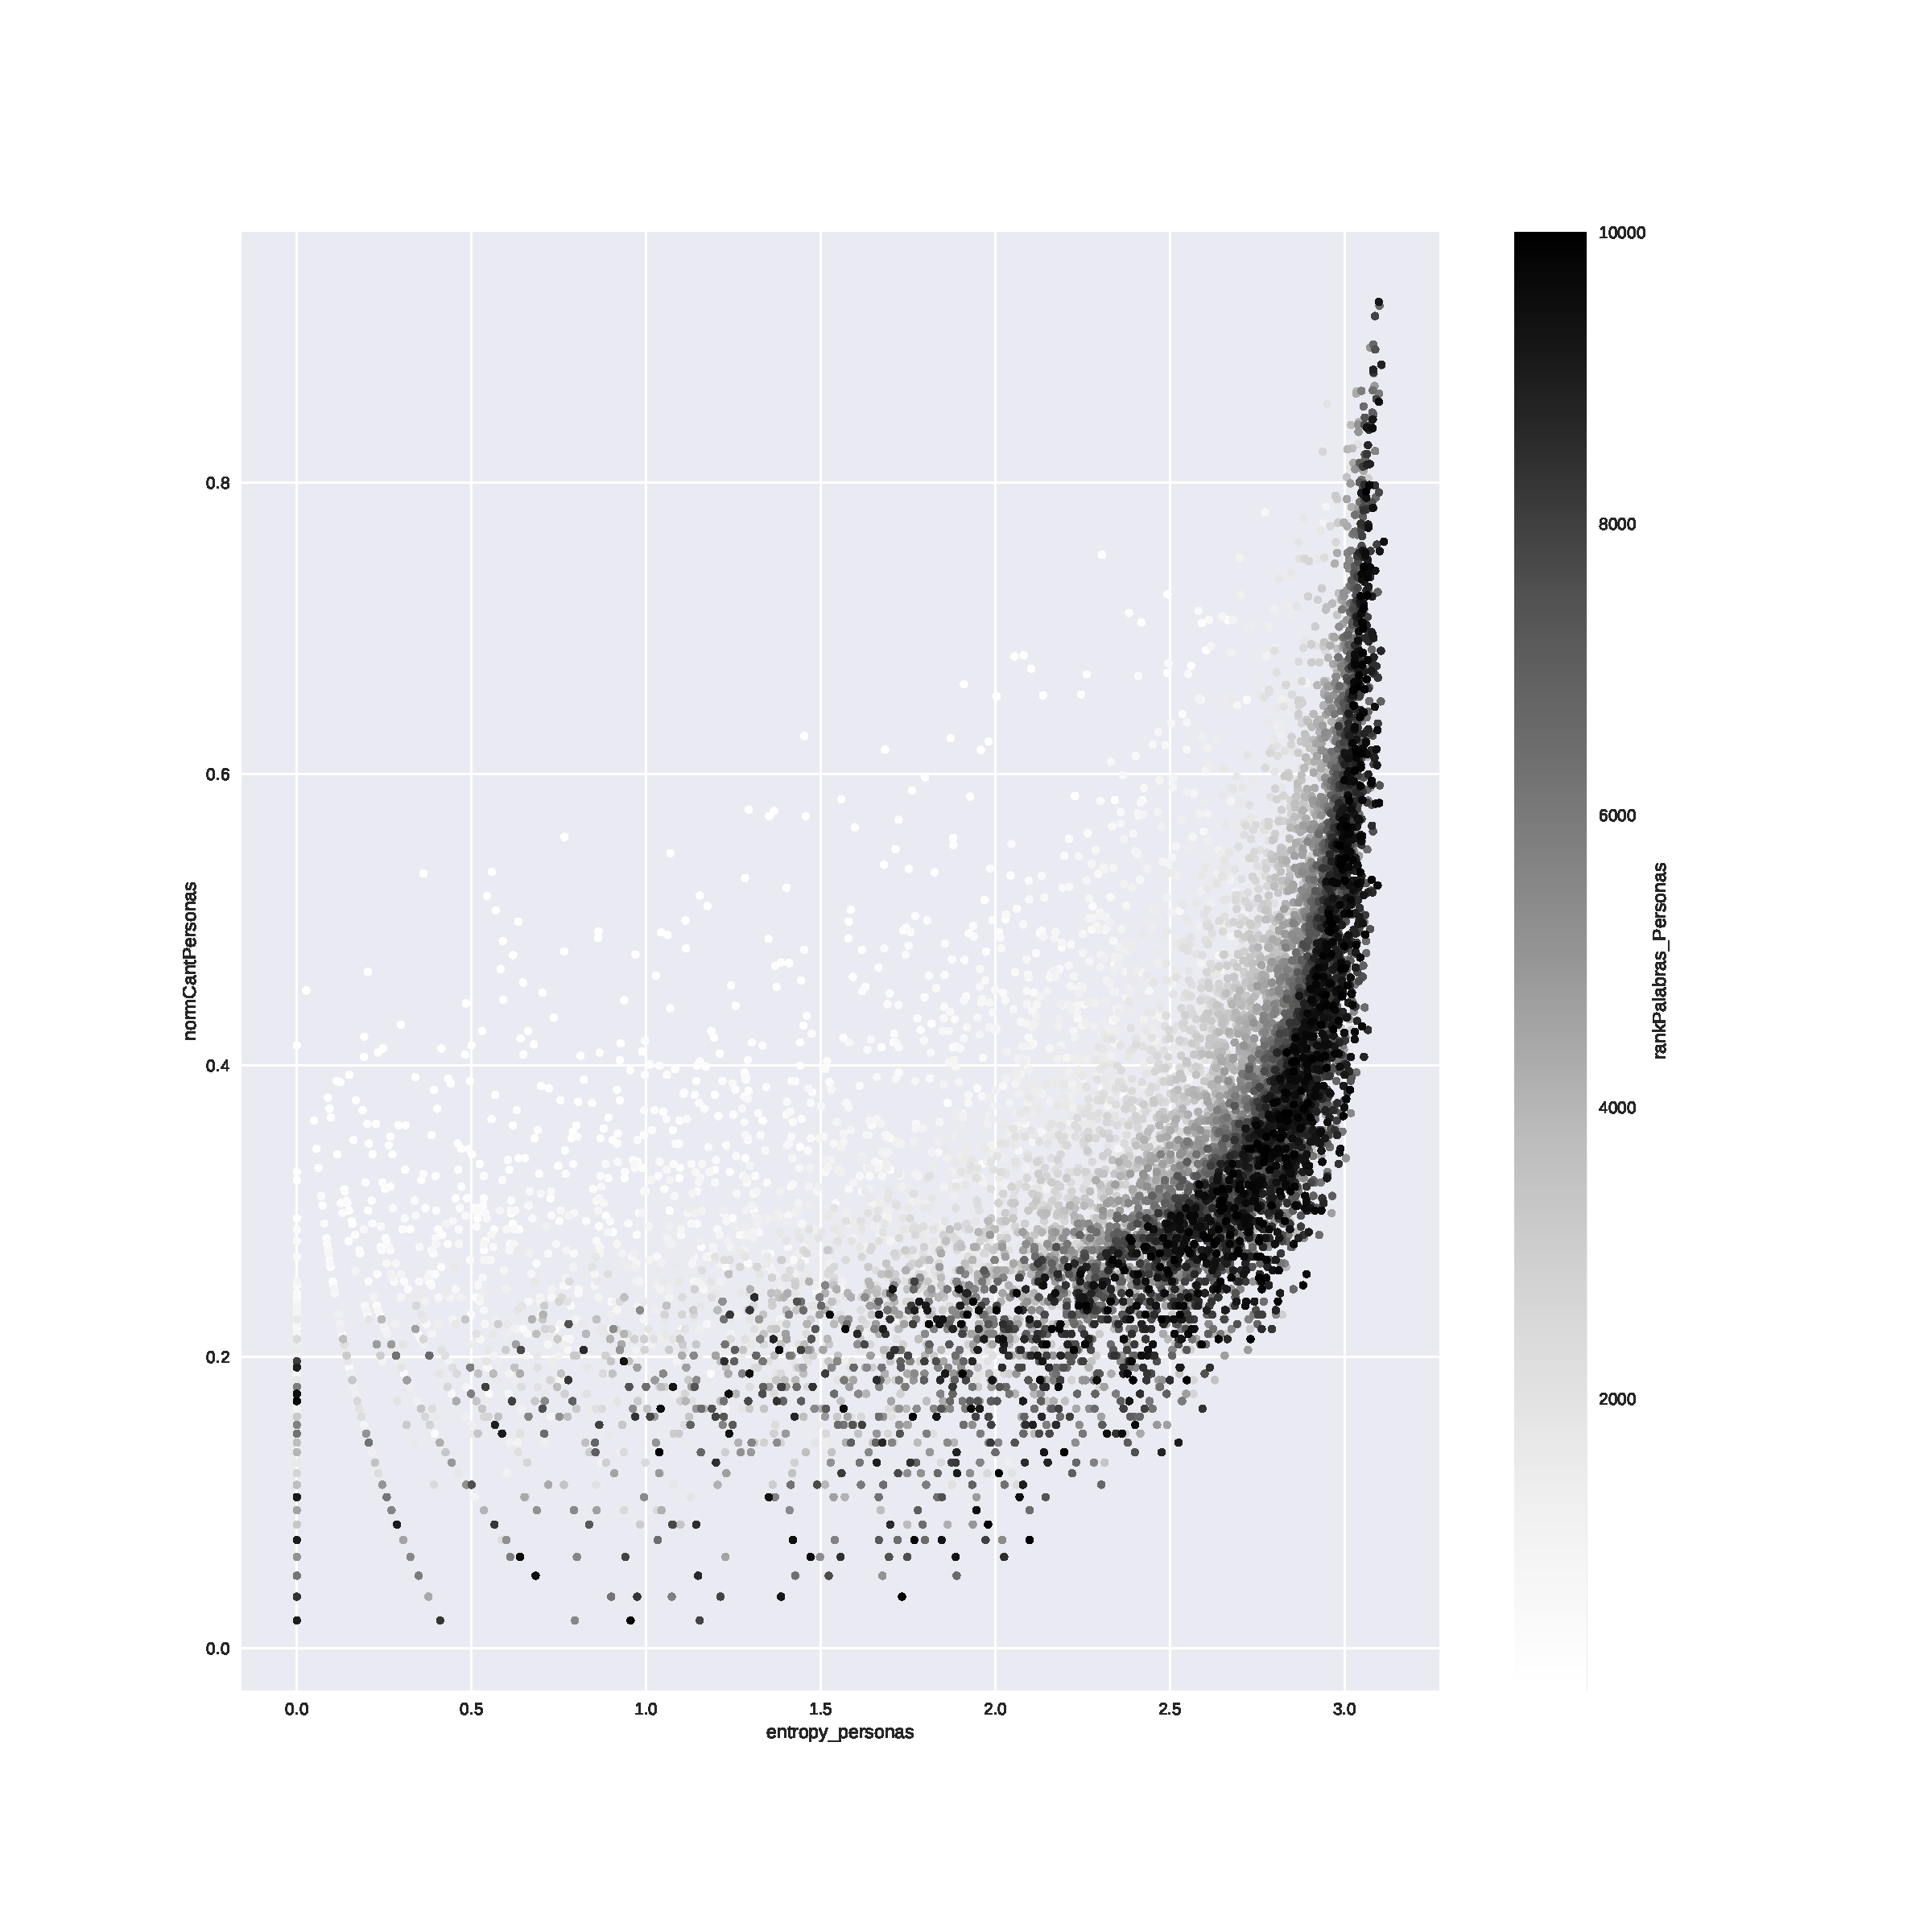
\includegraphics[width=1.0\textwidth]{./images/entropiaPersonasxNormCantPersonas.pdf}
\caption{Gráfico de dispersión que muestra la posición en el listado ordenado según el valor de la información a partir de la escala cromática. Las posiciones más bajas aparecen más blancas. A su vez se muestra para cada palabra el valor de la entropía de las personas ($H_u$) y la cantidad normalizada de personas que utiliza dicho término($norm_p$). } 
\label{fig:infoValue} 
\end{figure}

En la figura \ref{fig:ivalue} se puede ver el valor de la información según la posición en la que se encuentra en el listado ordenado por la métrica. Notamos que el valor se estabiliza aproximadamente a partir de la palabra cuya posición es 4000 acercándose a 0.


\begin{figure}[!ht]
\centering
\includegraphics[width=1\textwidth]{./images/train/conFiltro/valorInformacionCorte.pdf}
\caption{Distribución del valor de la información según la posición de la palabra en el listado de palabras. El gráfico se realizó sobre el conjunto de palabras cuya cantidad de ocurrencias era mayor a 40 y la cantidad de usuarios que utilizaron cada término era mayor a 5. } 
\label{fig:ivalue}
\end{figure}


\section{Proporción acumulada de ocurrencias} % (fold)
\label{proporcionDeOcurrencias}

Para tener una mejor noción sobre la métrica, medimos el porcentaje de las ocurrencias de las palabras que muestran contrastes según nuestra métrica cubiertas por subconjuntos de provincias de manera tal que para cada palabra y un número fijo de provincias, la región con esa cantidad de provincias tenga un cubrimiento máximo. 
En la figura \ref{fig:propAcum} mostramos la proporción acumulada de las palabras, tomando diferentes muestras de palabras. Es notable la diferencia de proporciones acumuladas según la muestra de palabras. Solamente con una provincia para cada palabra ya se puede cubrir, en promedio, el 76\% del total de ocurrencias sobre las mil palabras con mayor valor de la información.

%TODO: cambiar el grafico con todas las palabras candidatas OK
En el gráfico \ref{fig:propAcum5000} se observa que la variación del cubrimiento de ocurrencias es menor a medida que se aumenta la cantidad de provincias. 


\begin{figure}\centering
    \includegraphics[width=1\textwidth]{images/PropAcumSinCandidatas.pdf}
    \caption{Proporción de ocurrencias acumulada según la muestra de palabras.} 
    \label{fig:propAcum} 
\end{figure}


\begin{figure}\centering
    \includegraphics[width=1\textwidth]{images/PropAcum5000SinCandidatas.pdf}
    \caption{Variación de la proporción de ocurrencias acumulada a partir de la muestra con las primeras 5000 palabras con mayor valor de la información.} 
    \label{fig:propAcum5000} 
\end{figure}



\section{Análisis de las palabras contrastivas encontradas}
\subsection{Caracterización de las palabras identificadas como contrastivas}

\begin{frame}[t]\frametitle{Palabras candidatas}

    \begin{columns}
        \begin{column}{.5\textwidth}
        Para buscar las palabras candidatas a tener contrastes significativos en cuanto a la cantidad de ocurrencias en distintas provincias, elegimos el conjunto de las primeras 
        cinco mil (5000) palabras con mayor valor de nuestra métrica.

        \end{column}

        \begin{column}{.45\textwidth}
            \begin{figure}
            \centering
            \includegraphics[width=0.95\linewidth]{../src/images2/valorInformacionCorte.pdf}
            \label{fig:ivalue}
            \end{figure}
        \end{column}
    \end{columns}

\end{frame}

\begin{frame}[t]\frametitle{Validación lingüística}

   \begin{itemize}

      \label{it:caracterizacionLinguistica}

      \item \textbf{Coloquialismos o vulgarismos}

      \blockquote[Córdoba]{Perdon pero tenes que ser muy \textbf{culiado/a} para ir a mc y pedirte una ensalada}


      \blockquote[Mendoza]{Q \textbf{chombi} hacer un chiste y q la otra persona no se ría o no lo entienda}

      %   \blockquote[Neuquén]{Que \textbf{carnasas} poniendole rosas rojas a toda la ropa, para mi queda horrible sorry}

      %   \blockquote[Chaco]{Teres, \textbf{pororós} y pelis con Carlita y Flor}

      % \blockquote[San Juan]{Ver un negro \textbf{chuño} con musculosa y gorro.. se ve que el tipo no quería pasar ni frío ni calor.}

      % \blockquote[Formosa]{Tenía la re expectativa para este sábado y al final \textbf{trancó} todo }

      \item \textbf{Indigenismos}

      \blockquote[Formosa]{Te regalo ser \textbf{mitaí} y ir a jurar la bandera con el guardapolvo caliente ese y la corbata que te ahorca todo (Del guaraní mitaí “pequeño”)}

      \blockquote[Corrientes]{\textbf{Angá} mi negrito, esta triste (Del guaraní angá aprox. “pobre”)}

      \item \textbf{Gentilicios}

      \textbf{Casildense} (de Casilda), \textbf{concordiense} (de Concordia) y \textbf{obereño} (de Oberá).

\end{itemize}

% \item \textbf{Voces no marcadas en registro, que aluden a una realidad local}

%   \blockquote[San Juan]{Quiero a alguien que me diga vamos a comer \textbf{piadinas}, un pancho, un chori, una hamburguesa lo que sea y soy feliz}

%   \blockquote[Misiones]{\textbf{Tareferos} que reclamaban asistencia interzafra en Posadas estarían preparando una protesta para hoy en la Fiesta del Inmigrante en Oberá.}

%   \blockquote[Jujuy]{Me encantan los bohemios anti sistema que usan vans. Es como que seas ecologista y uses un cuaderno hecho con media \textbf{yunga}.}

\end{frame}

\begin{frame}[t]\frametitle{Más resultados}
    

\begin{itemize}
  
\item \textbf{Leísmo}

  \blockquote[Misiones]{No te olvides de \textbf{saludarle} a tu suegro hoy}

  \blockquote[Misiones]{Vine a \textbf{visitarle} a mis primas y estan re colgadas, para eso me quedaba en mi casa no maaa }

  \blockquote[Formosa]{A \textbf{esperarle} a nahuel, que traiga los teresss }

% \item \textbf{Fusiones y acrónimos que pueden señalar pronunciación o alta frecuencia de uso}

%   \blockquote[Buenos Aires]{Los sueños de la siesta me dejan \textbf{patra} }

%   \blockquote[Córdoba]{Si mañana me dice q no, voy sola, necesito ver esa pelicula en el cine siosi}

% % \item \textbf{Voces consideradas generales pero que, al aparecer en la lista, permitieron verificar su contrastividad en frecuencia de uso al menos con respecto a España}
%   % Ejemplos: \textbf{pavada}, \textbf{distrital} y \textbf{cariño}.

\item \textbf{Voces sospechadas generales pero con acepción local diferente}

  \blockquote[Mendoza]{Mañana que alguien \textbf{atine} con parque y porrones}

  \blockquote[San Juan]{\textbf{Mansas} ganas de sentarme a tomar un te con semitas}

  \blockquote[Tierra del Fuego]{\textbf{Habilítenme} una nueva espaldaa}

  \blockquote[San Juan]{sigo \textbf{asada} por cosas que han pasado hace como dos dias, que falla (Mendoza) / Que \textbf{asada} estoy, tengo la cabeza echa un lío}


\item \textbf{Voces con una morfología propia de una región}

Ejemplo: terminación azo/aza con base adjetiva.

  \blockquote[San Juan]{Creo que va a estar \textbf{malazo} lo de esta noche } 

  \blockquote[Córdoba]{Esta \textbf{locaza} esa mina para hacer eso}

% \item \textbf{Variantes ortográficas}

%   Ejemplos: culiado (adj. despect. o fórmula de tratamiento de confianza) y tereré.

%   \blockquote[Tucumán]{Menos mal que soy de los chetos de la carne y mañana tengo \textbf{asao} todo el dia jajajajaj}

%   \blockquote[Catamarca]{Un lunes con buen humor ta \textbf{pasao} }

%   \blockquote[Corrientes]{Ahora a la mañana tengo q ir hacerme la tarjebus jajajajj \textbf{mavale} q me estoy por levantarrr jajajaj}  

%   \blockquote[Córdoba]{Q paja volver al colegio \textbf{culiaa}}

%   \blockquote[Córdoba]{Que pajero el \textbf{qliao} este.}

%   \blockquote[Córdoba]{Quiero recitaaal \textbf{qliaaaa}}

%   \blockquote[Entre Ríos]{\textbf{Tereresss} y pile con todos mis primisss}

%   \blockquote[Corrientes]{No se si hacerme un \textbf{tere} o un mate para pasar la siesta}

%   \blockquote[Chaco]{Es lo mas lindo no ir al colegio y quedarme a tomar \textbf{teresss}}


% \item \textbf{Formas verbales coloquiales con sustantivos o adjetivos como base}

%   \blockquote[Neuquén]{Me calma mucho \textbf{mimosear} a mi perro }

%   \blockquote[Buenos Aires]{Me vine a acostar y ya me dicen que parezco de 80 años ME CHUPA UN HUEVO LO QUE PIENSEN, DEJENME \textbf{ABUELEAR} }

%   \blockquote[Tierra del Fuego]{Estaría bueno que ari venga aunque sea a saludarme y que no se quede todo el tiempo \textbf{pollereando}.}


% \item \textbf{Vesres}: Creación de palabras por inversión de sílabas que se usa jergalmente o con fines humorísticos.

%   \blockquote[Corrientes]{Estoy en lo de villa mateando con él y jimmy. Pinta \textbf{sogui} abundante más tarde dijeron }

%   \blockquote[Chaco]{Uhhh me acuerdo si no habré saltado el muro del aguapey par colarme a los \textbf{cequin}. (cequín “fiesta de quince”)}

% \item \textbf{Intejercciones}

%   \blockquote[Formosa]{\textbf{Aijué}, encima me decís vieja, re que no pinta esto facundo jaja ya te dije como es la onda, fin }

%   \blockquote[Formosa]{\textbf{Ains}, una mujer hablando de fútbol.}

%   \blockquote[Corrientes]{Al fin una buena: hora libreeee! \textbf{Yirr} }
% \end{itemize}

\end{itemize}
\end{frame}


\subsection{Validación estadística}

\begin{frame}[t]\frametitle{Problema desde el punto de vista estadístico}


    


\end{frame}

\begin{frame}[t]\frametitle{Test hipergeométrico}

    Para aplicar el test hipergeométrico representamos los datos sobre la palabra en una tabla de 2x2 como la de la siguiente Tabla.

    \begin{table}[ht]
    \centering
    \begin{tabular}{l|ccc}
    \hline
    &  \begin{tabular}{@{}c@{}}\#Palabras \\sobre región\end{tabular} &  \begin{tabular}{@{}c@{}}\#Palabras en el \\ resto de Argentina\end{tabular}  &Total \\ \hline
    \# Palabras w &   $k$ & $K-k$ & $K$ \\ 
    \# Palabras $\neq$ w & $n-k$ & $N + k - n - K$  & $N - K$ \\ \hline
    Total & $n$ & $N -n$ & $N$ \\ 
    \end{tabular}
    \label{tab:contingencia}
    \end{table}

\end{frame}

\begin{frame}[t]\frametitle{Test t de Welch}

    El test de Welch nos provee un valor de probabilidad para rechazar la hipótesis nula que afirma que las medias de las dos distribuciones son iguales.

    \only<2>{
       Las suposiciones del test 
        \begin{enumerate}
            \item Todos los textos son estadísticamente independientes 
            \item La media de las frecuencias proviene de una distribución normal
        \end{enumerate}
       } 
    
    \only<3>{
       \begin{block}{Metodología}
              Agrupamos todos los tuits de cada usuario representando un texto.\footnote{Notar que la suposición de independencia es más débil.}
        \begin{description}
            \item[Corpus S] Todos los textos de los usuarios que provienen de las provincias en donde se cubre el 80\% de las ocurrencias
            \item[Corpus T] Los textos creados por usuarios del resto de las provincias
        \end{description}

        \end{block}
       }
\end{frame}


\begin{frame}[t]\frametitle{Resultados test t de Welch}

  \begin{enumerate}
    \alert<1>
    {
    \item Para cada métrica $I,I_W,I_P$  variamos los subconjuntos de palabras de acuerdo al listado ordenado según estas.
    }
    
    \alert<2>
    {
    \item Calculamos la tasa de rechazo de la hipótesis nula, definida por:
    \begin{equation}
      \text{Tasa de rechazo(tests)} = \frac{\# \{t:tests \mid p-valor(t) < 0.05\}}{\#tests} 
    \end{equation}
    } 
  \end{enumerate}

  \begin{figure}
  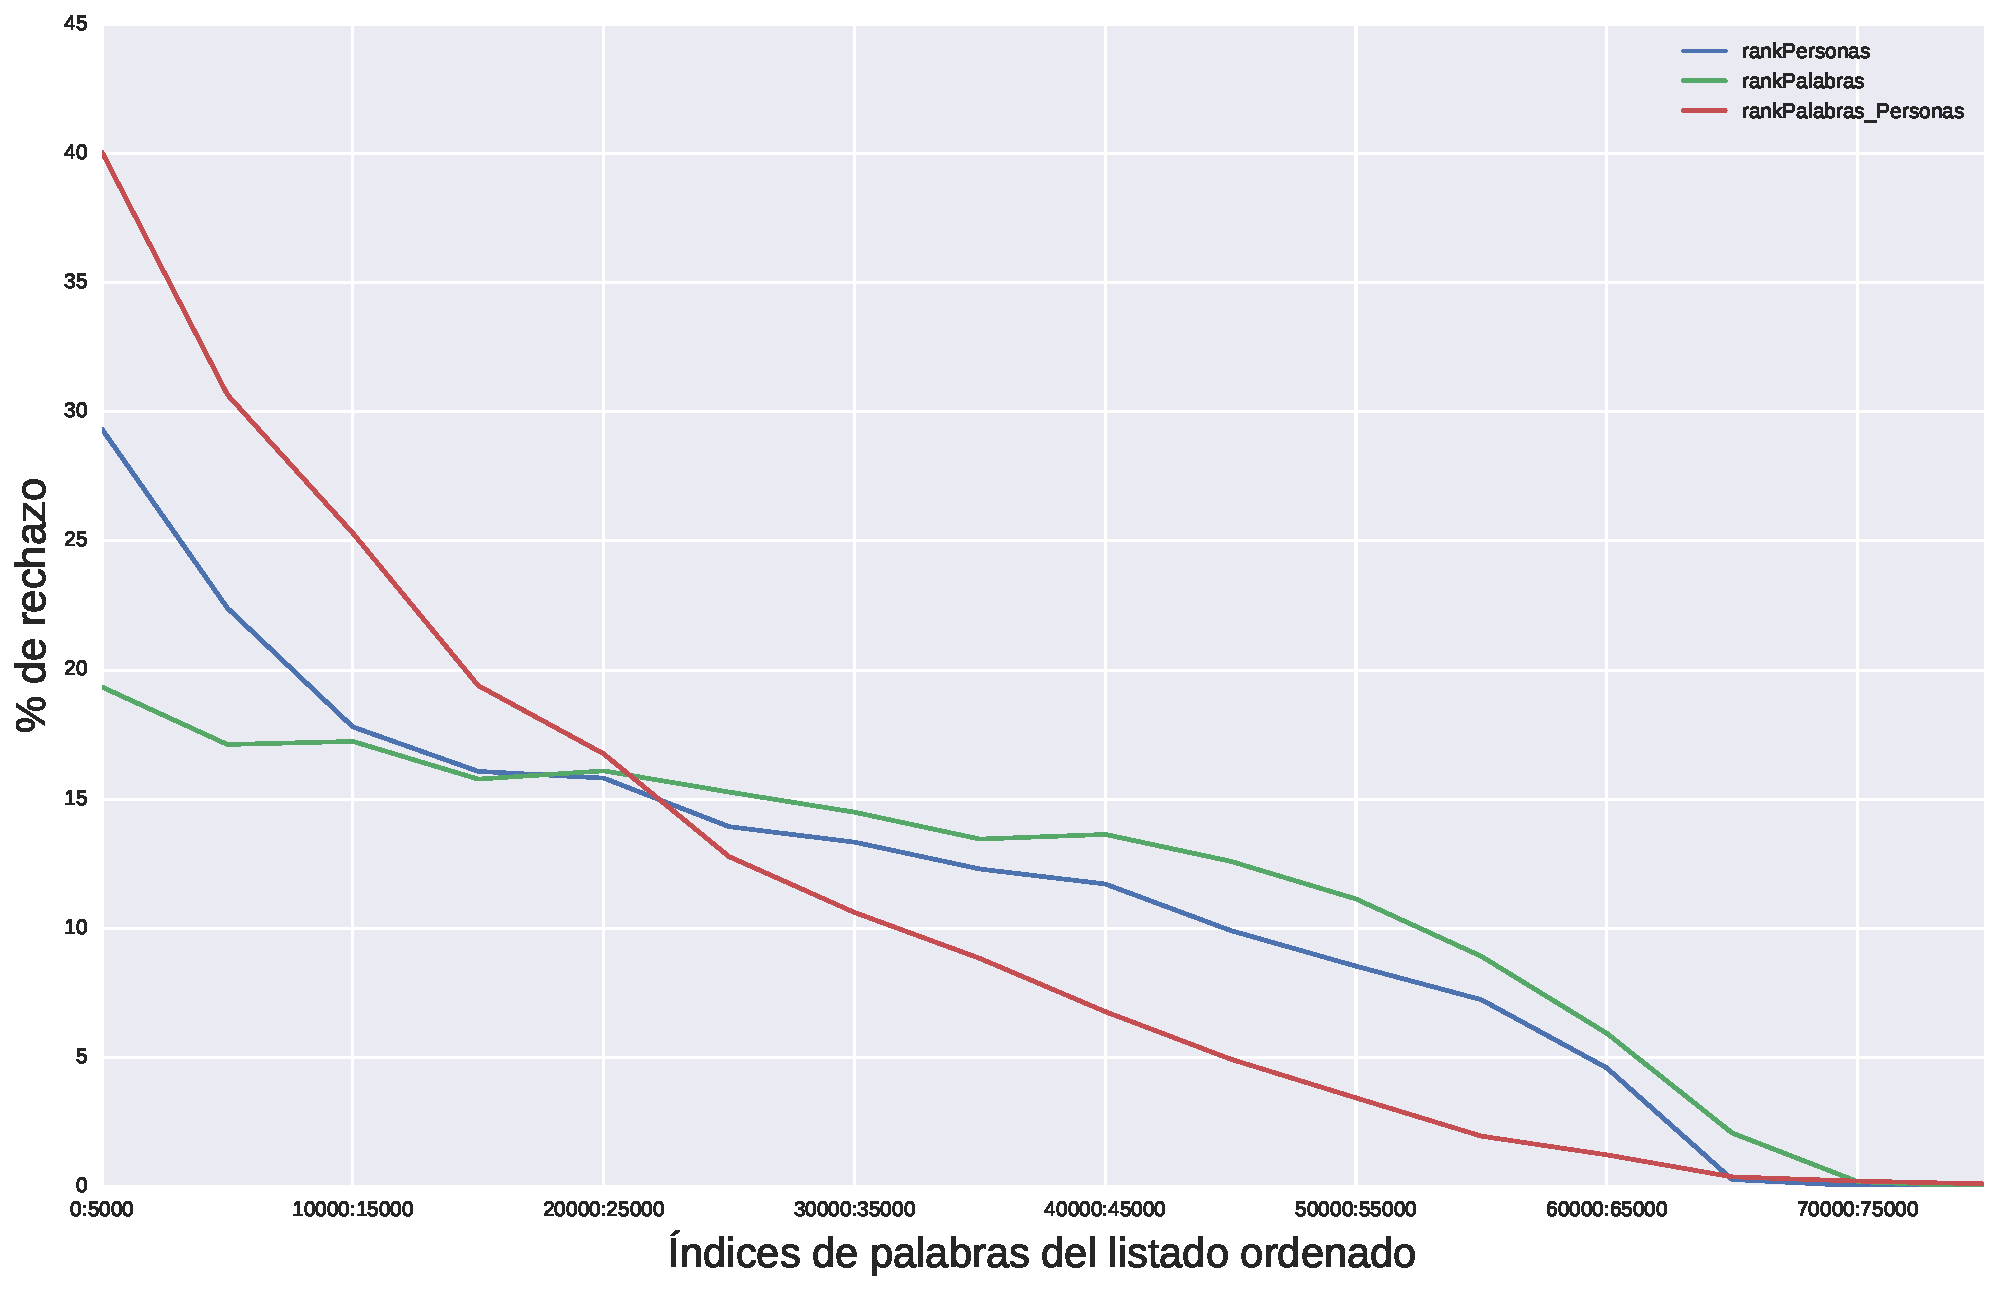
\includegraphics[width=0.50\linewidth]{../src/images/rechazo_metricas.pdf}
            % \label{fig:rechazo_metricas} 
  
  \end{figure}
            
\end{frame}

\section{Conclusiones y trabajo futuro}
\begin{frame}[t]\frametitle{Conclusiones}
    
    \begin{itemize}
        \item Desarrollamos una métrica de la contrastividad de uso de una palabra en distintas regiones.
        \item Para probar esta métrica recolectamos un conjunto de datos de textos de la Argentina a través de la API de Twitter.
        \item Obtuvimos aproximadamente 1 palabra contrastiva relevante lingüísticamente cada 17 palabras.
        \item Varias de las palabras detectadas a partir de la métrica desarrollada serán agregadas al Diccionario del habla de los argentinos.
    \end{itemize}

\end{frame}

\begin{frame}[t]\frametitle{Trabajo a futuro}
    
    \begin{itemize}
        \item Reproducir el trabajo para todos los países hispanoparlantes.
        \item Obtener regiones dialectales a partir de métodos de clustering, lo cual permitiría validar la vigencia de las regiones propuestas por Vidal de Battini en 1964 \cite{vidal1964espanol}.
        \item Analizar la contrastividad léxica comparando la distribución de n-gramas.
    \end{itemize}

\end{frame}

\begin{frame}[t]\frametitle{¿Preguntas?}
    
\end{frame}

\bibliographystyle{alpha}
\bibliography{presentacion}
\end{document}